\chapter{Data Analysis II}

\section{Radio Isotope Beam Factory (RIBF) Facility }
\label{sec:beam}
%Cyclotron facility overview.
%Samurai line overview.
%Beam line element overview.
%Big rips beam PID. reference 
The primary and secondary beams were produced at the Radioactive Isotope Beam Factory (RIFB) facility at RIKEN, in Wako-shi, Japan. The RIBF facility starts with two primary beam types, ${}^{132}$Xe and ${}^{238}$U, which are produced by an ion-source and accelerated to progressively higher kinetic energies by 1 linear accelerator (RILAC), and 4 different cyclotrons (RRC, fRC, IRC, and SRC), until they reach a beam energy of \SI{345}{\MeVA}. Figure~\ref{fig:samuraiBeamLine} shows the later stages of the cyclotrons and the following beam lines they feed into.

\begin{figure}[!htb]
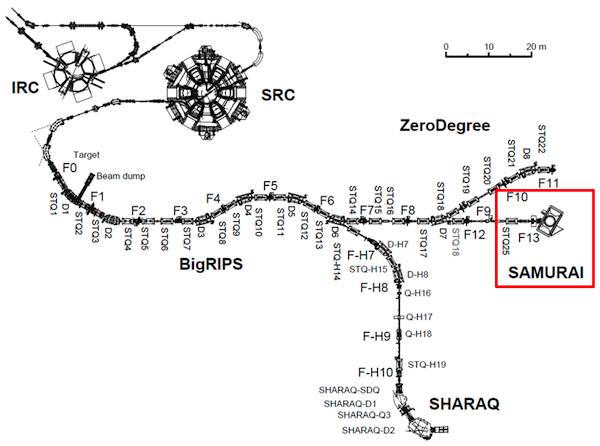
\includegraphics[width=\linewidth]{SAMURAI-beamline.png}
\caption{Overview of the RIBF, BigRIPS, and SAMURAI beamline.}
\label{fig:samuraiBeamLine}
\end{figure}

After the SCR, the primary beams impinge on a rotating \SI{3}{\milli\metre} Be target which produces many different species by fragmentation. These fragments are then separated by the BigRIPS spectrometer which is tuned to the particular secondary fragment of interest. This is accomplished through several dipole magnets, slits, and wedge degraders. The resulting secondary beam is not pure and the purity depends on the capability of BigRIPS to deliver the secondary beam of choice and the primary beam used. 

In these set of experiments several beams were produced with varying intensities and purities. Table~\ref{tb:beams} summarizes the average qualities of the 4 secondary beams produced in the two experimental campaigns where most beams were delivered with an intensity of \SI{10}{\kilo\hertz}. 

 \begin{table*}\centering
\ra{1.3}
\begin{tabular}{@{}ccccc@{}}\toprule 
 Primary Beam & Secondary Beam & Energy at mid target \si{\MeVA} & Intensity \si{\kilo\hertz} & Purity (\%) \\ [0.5ex] 
 \midrule
 ${}^{238}$U   & ${}^{132}$Sn   &  269.2  &  9.5  &  54   \\
 ${}^{238}$U   & ${}^{124}$Sn   &  270.3  &  9.1  &  10  \\
 ${}^{124}$Xe  & ${}^{112}$Sn   &  270.4  &  7.6  &  48  \\
 ${}^{124}$Xe  & ${}^{108}$Sn   &  269.3  &  7.5  &  52   \\
 \bottomrule
\end{tabular}
\caption{Primary and secondary beam properties produced in the \spirit TPC experimental campaigns. }
\label{tb:beams}
\end{table*}


\section{Beam Particle Identification}


\begin{figure}[!htb]
\centering
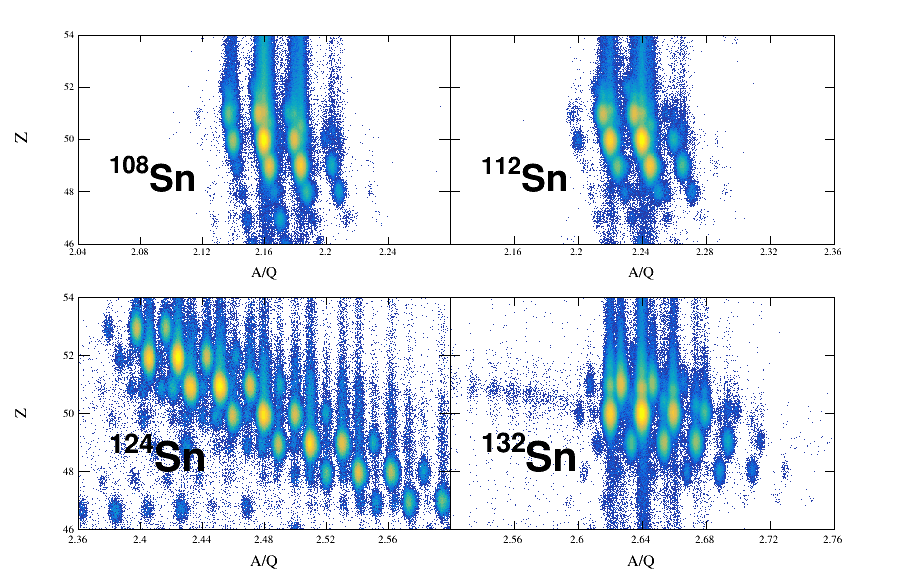
\includegraphics[width=\textwidth]{beamPID.png}
\label{fig:beampid}
\caption{Overall beam PID for all the systems. Several contaminants other than the desired secondary beam can be seen.}
\end{figure}


\begin{figure}[!htb]

     \centering
     \begin{subfigure}[b]{0.49\textwidth}
         \centering
         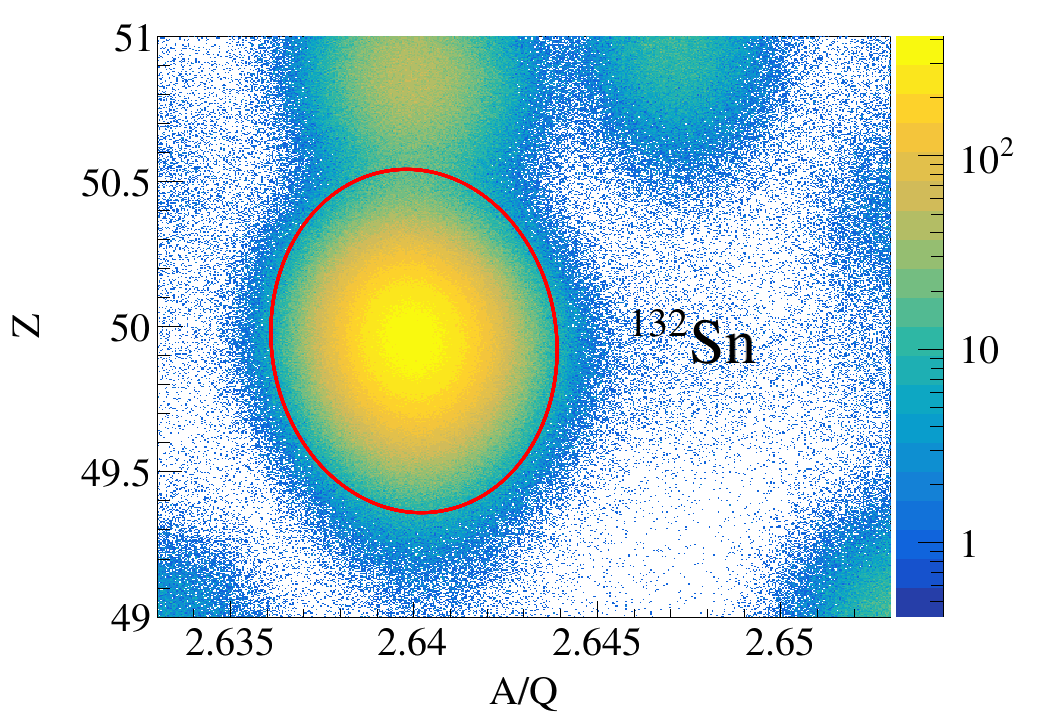
\includegraphics[width=\textwidth]{beam-Sn132.png}
         \caption{$\tin{132}{124}$ Beam particle identification.}
         \label{fig:beampid132}
     \end{subfigure}
     \hfill
     \begin{subfigure}[b]{0.49\textwidth}
         \centering
         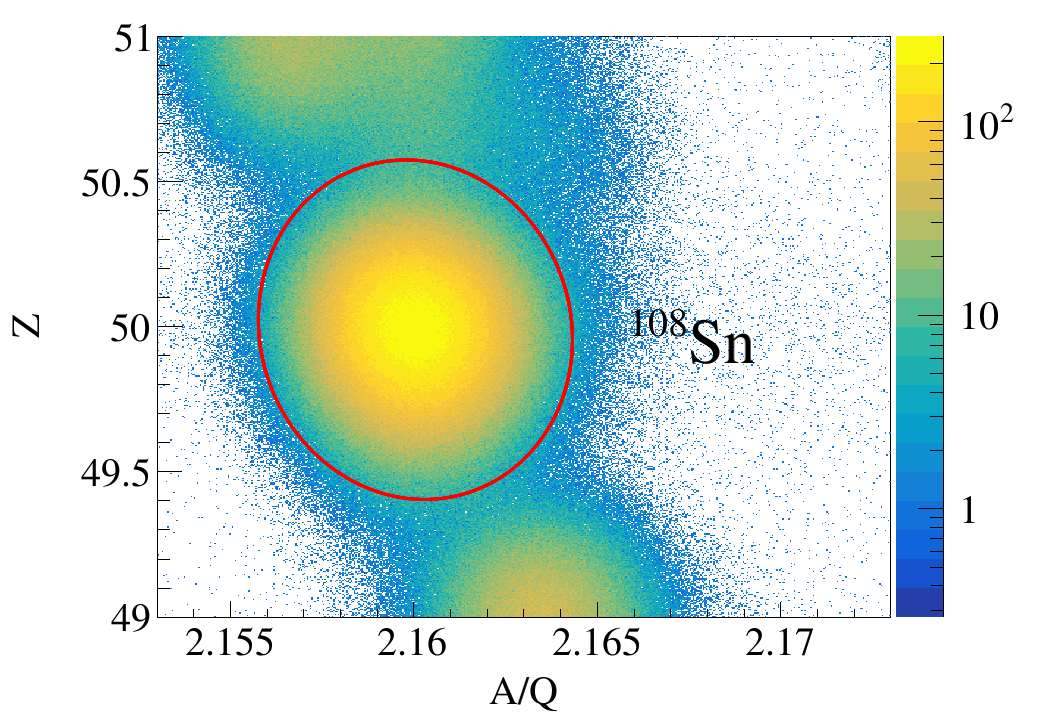
\includegraphics[width=\textwidth]{beam-Sn108.png}
         \caption{$\tin{132}{124}$ $\pi^-$ angular spectra.}
         \label{fig:beampid108}
     \end{subfigure}
        \caption{$\tin{108}{112}$ Beam particle identification. }
        \label{fig:beampidTwo}

\end{figure}


%Figures of beam contaminants in our beam PID line. 
%Table of beam purity reference to Jon's thesis paper
The secondary beam is produced through the projectile fragmentation of the primary beam off of a \SI{3}{\milli\metre} thick, rotating Be target \cite{inflightsep}. The resulting fragments are filtered in-flight to the desired seconary beam. The in-flight separation is handled by the BigRIPS fragment separator which is shown in Fig.~\ref{fig:samuraiBeamLine}. The dipole magnets D1 and D2 act as a velocity filter, selecting on certain magnetic rigidities $\beta\rho$. Several sets of slits further purify the secondary beam quality by throwing away particles which do not focus on the right focal planes. These are the areas where the particles with different velocities focus to different locations in space, which occur at F3,F5, and F7 positions.  Each beam is tracked with the remaining part of the BigRIPS spectrometer tracking system. The particle identification of each beam is achived by the TOF-B$\rho$-$\Delta$E method described in \cite{bigrips}, where the Time of Flight (TOF) information is given by the time it takes to cross two plastic scintilators at F3 and F7 focal planes, and the $\Delta$E information is given by the MUlti-Sampling Ionization Chamber (MUSIC) \cite{music}. From this method the atomic charge, Z, and mass to charge ratio, A/Q, of each particle was measured and separate species represent two-dimensional Gaussians in this space. 

Figure~\ref{fig:beampid} shows the beam PID for all the systems for events which satisfied the trigger, several contaminants other than the desired secondary beams still passed through the BigRIPS spectrometer and made it into the TPC. The beam purity of each desired secondary beam is listed in Table~\ref{tb:beams}. The desired secondary beam of interest can be selected by using an appropriate gate around the corresponding group, since the BigRIPS PID resolution is good enough to separate separate beam types. Each particle gate is selected by fitting a multivariate normal distribution with two variables defined as,

\begin{equation}
  f(x,y)=\frac1{2\pi\sigma_x\sigma_y\sqrt{1-\rho^2}}\exp\left\{
  \frac{-(x - \mu_{x})^2/\sigma_x^2-(y-\mu_{y})^2/\sigma_y^2+2\rho
  xy/\sigma_x\sigma_y}{2(1-\rho^2)}\right\},
   \label{multiGauss}
\end{equation}
where x=A/Q, y=Z, $\mu$ is the mean values, and $\sigma$ are the Gaussian widths of the two variables. The gates drawn in Fig.~\ref{fig:beampidTwo} are summarized in Table~\ref{beamParameters}. 

\begin{table}[H]
  \begin{center}
    \begin{tabular}{cccccc}
      \hline 
      Particle Type & $\mu_\mathrm{A/Q}$ & $\sigma_\mathrm{A/Q}$ & $\mu_\mathrm{Z}$ &
      $\sigma_\mathrm{Z}$ & $\rho$\\
      \hline\hline 
      ${}^{132}$Sn & 2.64 & 0.0014 & 49.95 & 0.209 & -0.052 \\
    %  $\tin{124}{112}$ & 2.24005 & 0.00150934 & 49.9906 & 0.194804 & -0.0671999 \\
    %  $\tin{112}{124}$ & 2.47995 & 0.00182327 & 49.961 & 0.214745 & -0.0742297 \\
      ${}^{108}$Sn & 2.16 & 0.0015 & 49.99 & 0.207 & -0.059 \\
      \hline
    \end{tabular}
    \caption{Multivariate normal distribution fit parameters for four beams.
    \label{beamParameters}}
  \end{center}
\end{table}
Figure~\ref{fig:beampid132} shows a zoomed in view of the PID centered around the ${}^{132}$Sn beam and Fig.~\ref{fig:beampid108} the ${}^{108}$Sn beam. The red lines represent the cut where particles identified inside the circle represent the beam events which are identified as the good beam events. For both ${}^{132}$Sn an ${}^{108}$Sn a 2.83$\sigma$ cut is taken around the mean values.  


\section{Edge Cuts}

\begin{figure}[!htb]

    \centering
    \begin{subfigure}[t]{0.45\textwidth}
        \centering
        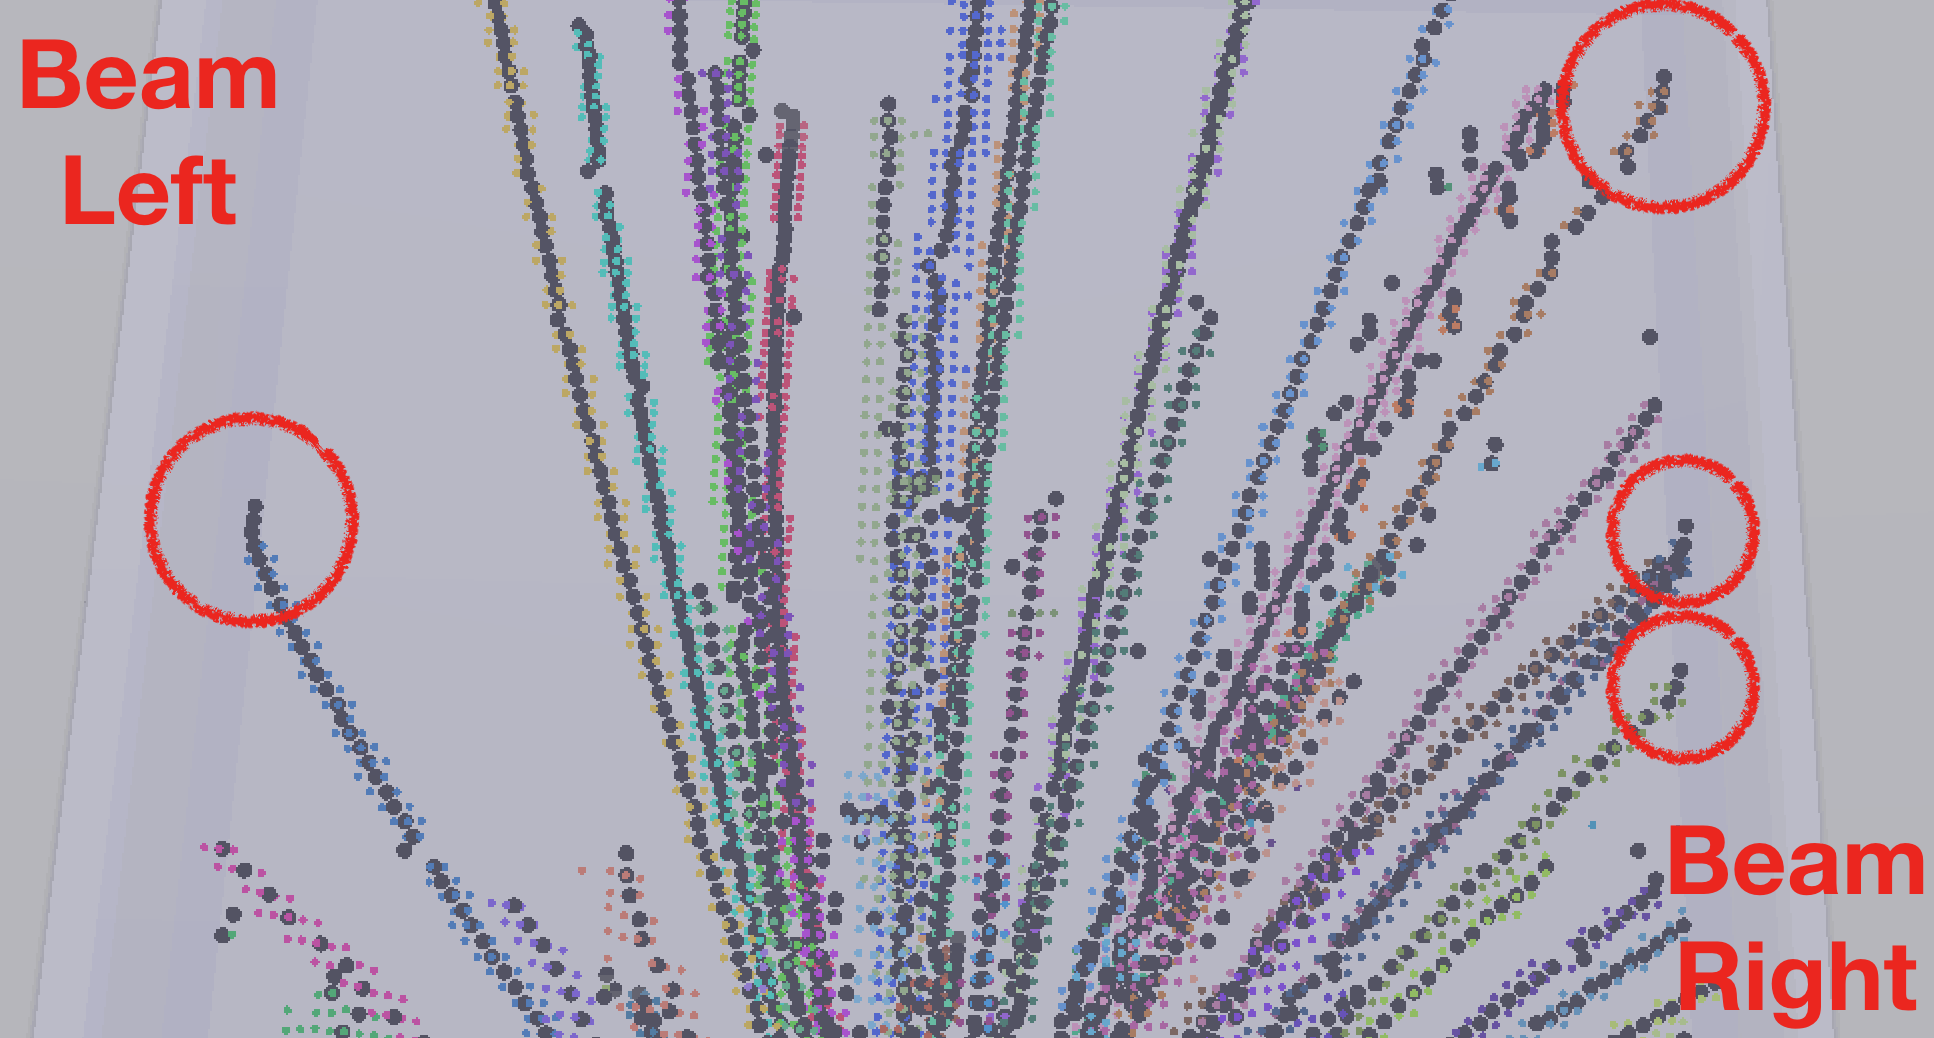
\includegraphics[width=\linewidth]{clusterLR.png} 
        \caption{Top view of the tracks showing the edge effect on the left and right sides of the TPC.} 	   \label{fig:clusterLR}
    \end{subfigure}
    \hfill
    \begin{subfigure}[t]{0.45\textwidth}
        \centering
        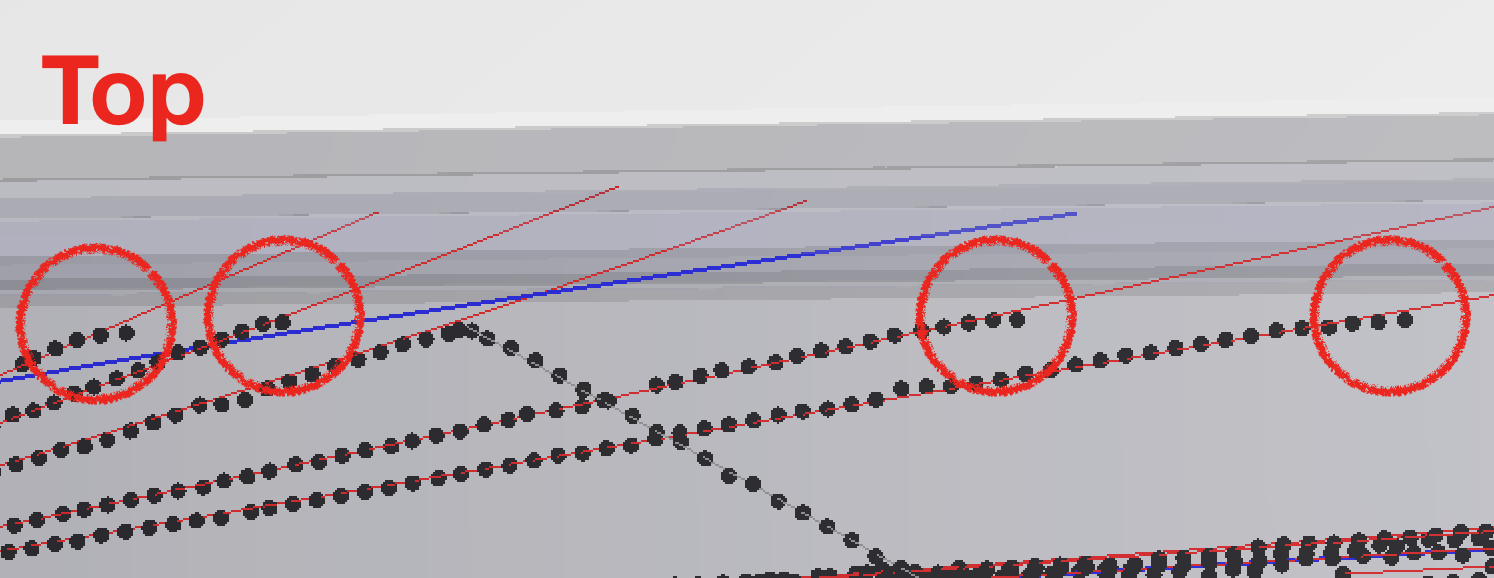
\includegraphics[width=\linewidth]{clusterTop.png} 
        \caption{Side view of the TPC showing the edge effect near the top.} \label{fig:clusterTop}
    \end{subfigure}
    
    \begin{subfigure}[t]{0.45\textwidth}
        \centering
        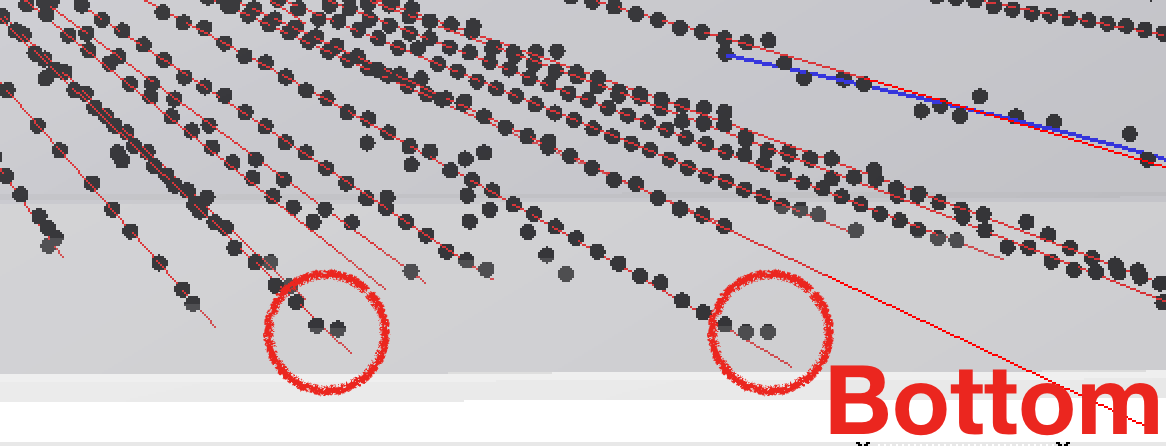
\includegraphics[width=\linewidth]{clusterBottom.png} 
        \caption{Side view of the TPC showing the edge effect near the bottom.} \label{fig:clusterBottom}
    \end{subfigure}
\caption{}    
\label{fig:edge}
\end{figure}

Near the edges of the detection volume, the clusters of tracks significantly deviate from the trend of the fitted track as seen in different view of the reconstructed clusters in Fig.~\ref{fig:edge}.  This effect comes from an edge effects where the last pads on the edges of the pad-plane have no neighboring pads containing charge, and therefore the last pad, or in the case of the vertical time bucket spectrum, represents the last known position of the collected charge. In this case the cluster position is biased towards the inside of the TPC. While the number of affected clusters is small as compared with the total number in the track, but the deviation at the end of the track is enough to start causing issues in the momentum reconstruction. Simple cuts were taken to graphically remove these clusters around the left,right, top, and bottom of the TPC. The hits that were cut out satisfied the following conditions, 

\begin{equation*}
  |x|\geq420~\mathrm{mm},\quad y\leq-522+\mathrm{y_o}~\mathrm{mm},
  \quad\mathrm{and}\quad y\geq-64+\mathrm{(Hit\ Shift)}~\mathrm{mm}.
\label{eq:hitshift}
\end{equation*}



\section{High Density Cut}


\begin{figure}[!htb]

     \centering
     \begin{subfigure}[b]{0.49\textwidth}
         \centering
         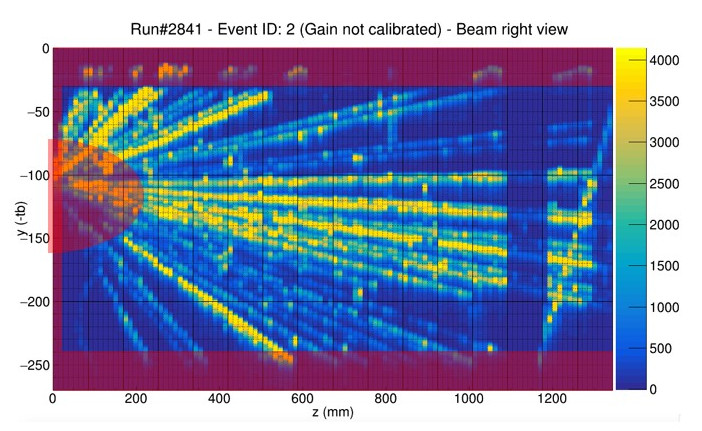
\includegraphics[width=\textwidth]{sideviewHighDenCut.jpg}
         \caption{Side view.}
         \label{fig:sideHigh}
     \end{subfigure}
     \hfill
     \begin{subfigure}[b]{0.49\textwidth}
         \centering
         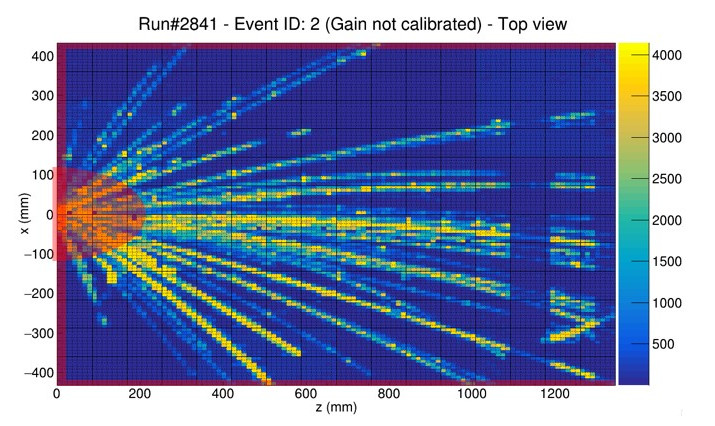
\includegraphics[width=\textwidth]{topviewHighDenCut.jpg}
         \caption{Top view.}
         \label{fig:topHigh}
     \end{subfigure}
        \label{fig:highcut}
        \caption{Views showing the high density and edge cuts.}
        \label{fig:elipsecut}
\end{figure}
The track multiplicity in each event is quite high and since the tracks all originate from a common vertex, the density of tracks near the target region is very high. In this region the track separation is too small for the software to correctly determine and sort the charge information into the appropriate track. The information provided by extra vertex point from external BDC tracking described in \ref{sec:bdc}, provides all the information about the vertex location. The bad quality of hit information near the target region only hurt in the tracking and PID of a track. Hits lying within an semi-ellipsoidal cut around the target are removed from the software and not included in the track and momentum reconstruction. Figure~\ref{fig:elipsecut} shows the extent of the ellipsoidal cut in the high density region, along with the edge cuts as shaded red regions in both views of the TPC. 

\section{Beam angle selection}
The incoming secondary beam is deflected by the magnetic field and impinges on the target at some small but significant angle. From the BDCs tracking information, the beam is projected as a straight line right up until entering the magnet.  The beam is then propagated through the magnetic field using a Runge-Kutta integration until reaching the target position. The beam angle on target can be categorized by two angles $\theta_{a_{proj}}$ and $\theta_{b_{proj}}$ defined as, 

%define angles 
%define selection

\begin{equation}
  \theta_\mathrm{a,proj}=\tan^{-1}\frac{p_x}{p_z},\quad
  \theta_\mathrm{b,proj}=\tan^{-1}\frac{p_y}{p_z},
  \label{beamAngle}
\end{equation}

where $p_x$, $p_y$, and $p_z$ are the components of beam momentum vector.



\begin{table}[H]
  \begin{center}
    \begin{tabular}{ccccc}
      \hline 
      System & $\mu_{\theta_\mathrm{a,proj}}$ &
      $\sigma_{\theta_\mathrm{a,proj}}$ & $\mu_{\theta_\mathrm{b,proj}}$ &
      $\sigma_{\theta_\mathrm{b,proj}}$ \\
      \hline\hline 
      $\tin{132}{124}$ & 0.61 & 2.94 & -44.18 & 1.96 \\
    %  $\tin{112}{124}$ & -0.41 & 1.58 & -53.52 & 0.90 \\
      $\tin{108}{112}$ & -0.42 & 1.95 & -55.17 & 0.97 \\
      \hline
    \end{tabular}
    \caption{2D Gaussian fit parameters for $^{132}$Sn, $^{112}$Sn and
      $^{108}$Sn beam angle. \label{beamAngleParameters}}
  \end{center}
\end{table}

\begin{figure}[!htb]
    \centering
    \begin{subfigure}[t]{0.45\textwidth}
        \centering
        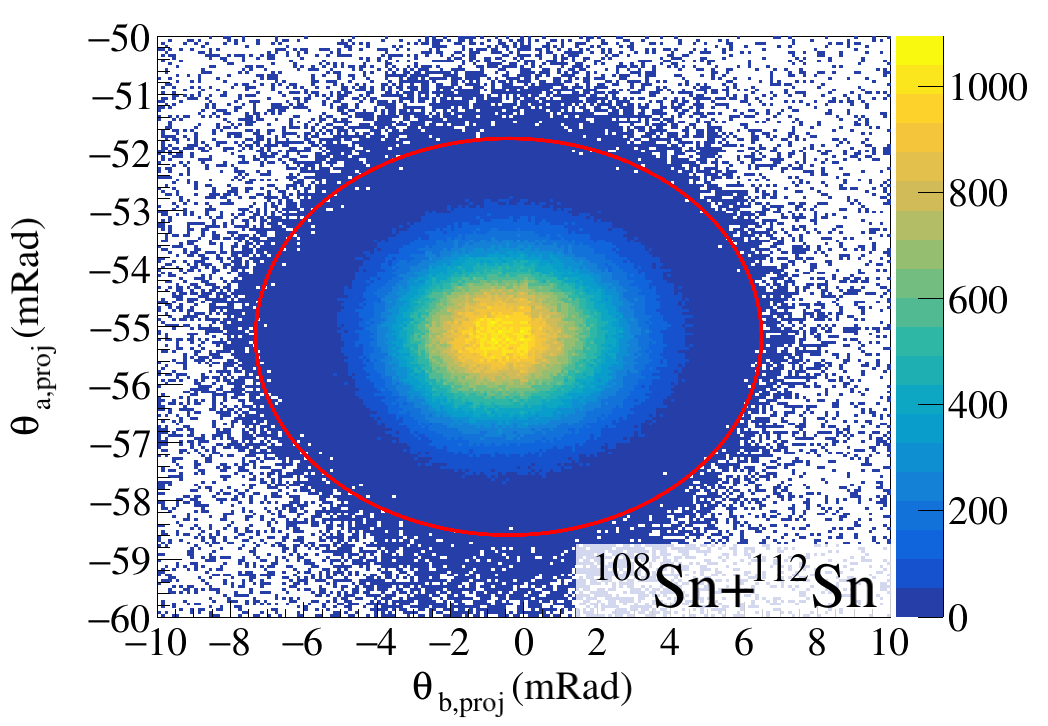
\includegraphics[width=\linewidth]{beamAngle-Sn108.png} 
        \caption{Beam angle of the $\tin{108}{124}$ system} \label{fig:beamangle108}
    \end{subfigure}
    \hfill
    \begin{subfigure}[t]{0.45\textwidth}
        \centering
        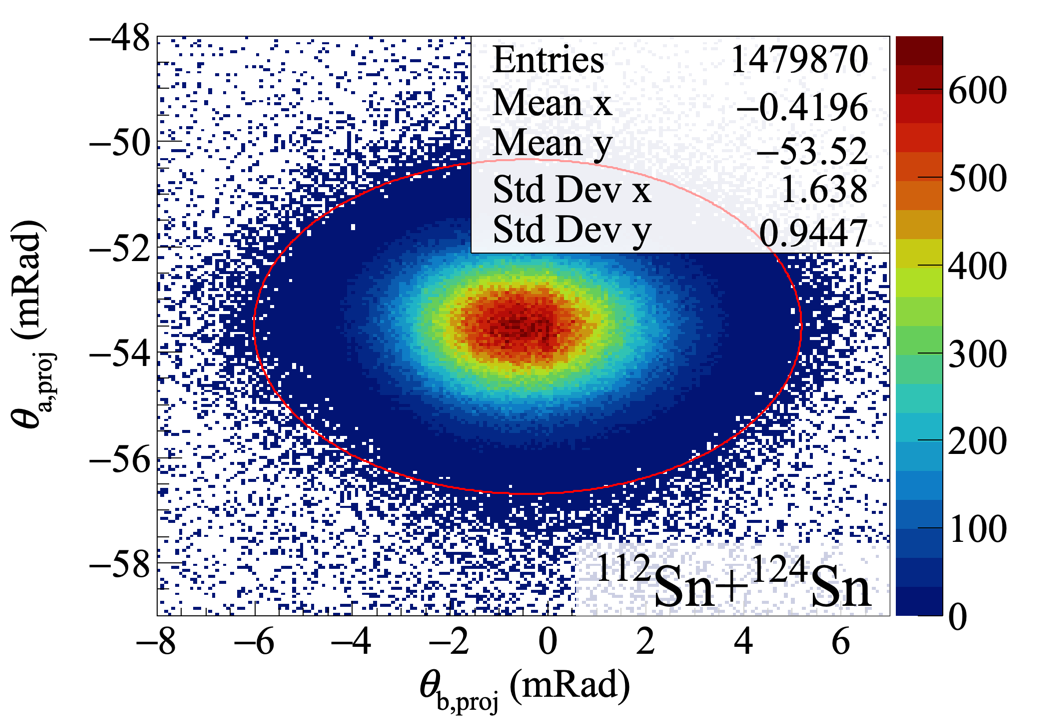
\includegraphics[width=\linewidth]{beamAngle-Sn112.png} 
        \caption{Beam angle of the $\tin{112}{124}$ system} \label{fig:beamangle112}
    \end{subfigure}
    
    \begin{subfigure}[t]{0.45\textwidth}
        \centering
        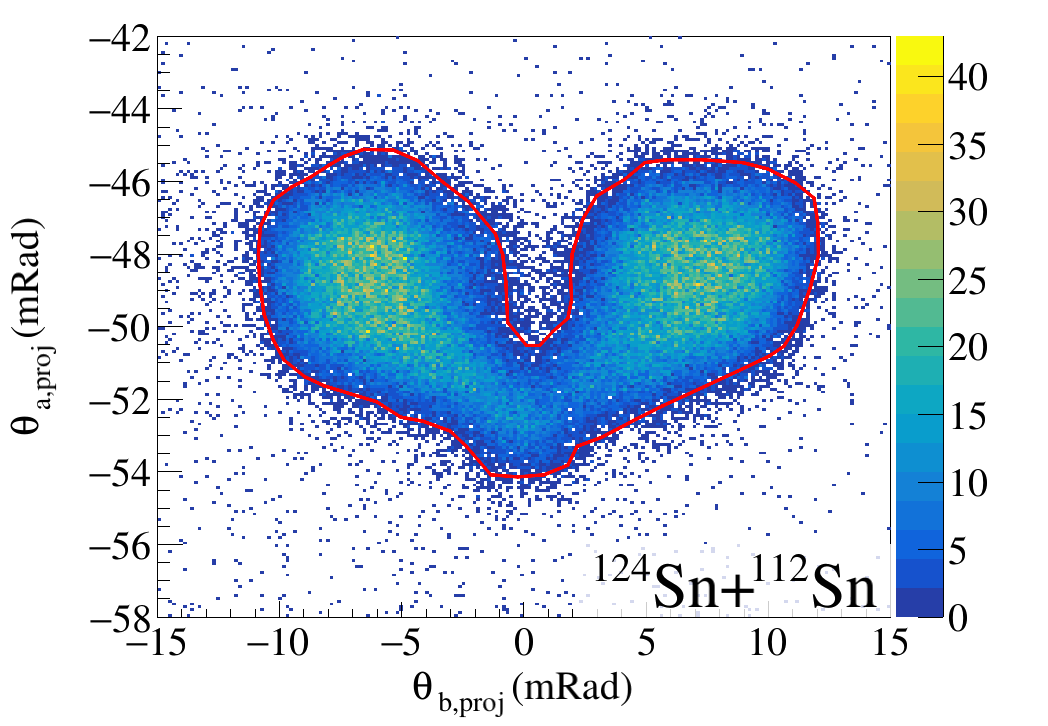
\includegraphics[width=\linewidth]{beamAngle-Sn124.png} 
        \caption{Beam angle of the $\tin{124}{112}$ system} \label{fig:beamangle124}
    \end{subfigure}
    \hfill
    \begin{subfigure}[t]{0.45\textwidth}
        \centering
        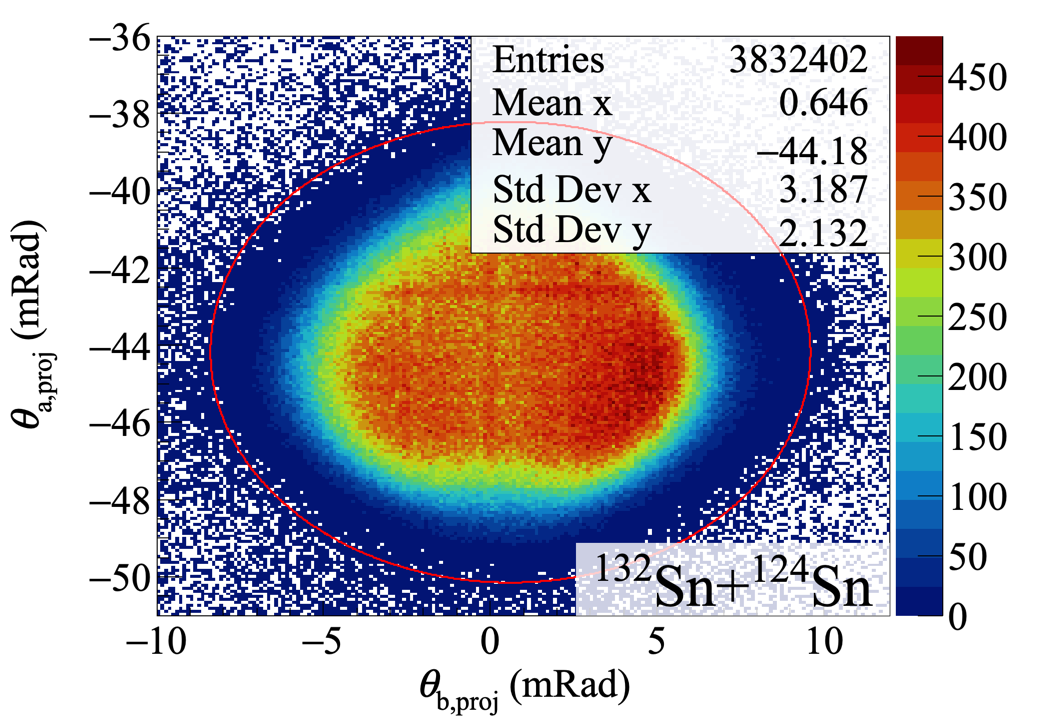
\includegraphics[width=\linewidth]{beamAngle-Sn132.png} 
        \caption{Beam angle of the $\tin{132}{124}$ system} \label{fig:beamangle132}
    \end{subfigure}
\label{fig:beamangle}
\end{figure}


Figure~\ref{fig:beamangle} shows the distribution of beam angles for ${}^{132}$Sn and ${}^{108}$Sn systems. Graphical cuts represented by the red lines where events lying in the cuts represent beams that were reconstructed correctly by the beam tracking software outlined in \cite{jon}. Helping to eliminate some of the poorly reconstructed beam events. 



\section{Vertex Cut}

\begin{figure}[!htb]
\centering
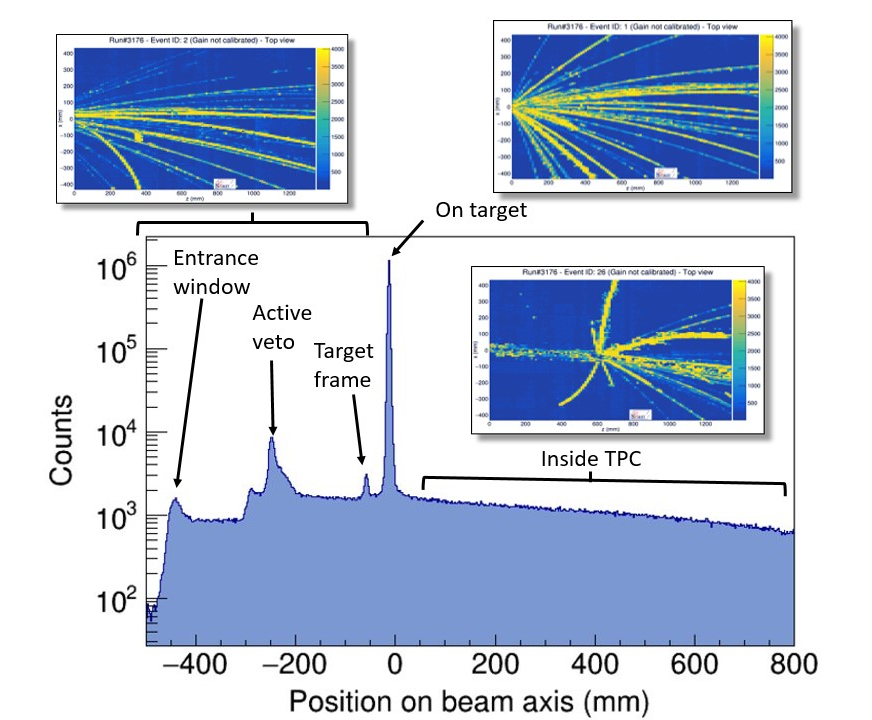
\includegraphics[scale =.5]{vertexDistribution.png}
\caption{Projection of the vertex onto the z-axis.}
\label{fig:overviewVertex}
\end{figure}


\begin{figure}[!htb]
\centering
    \begin{subfigure}[t]{\textwidth}
        \centering
        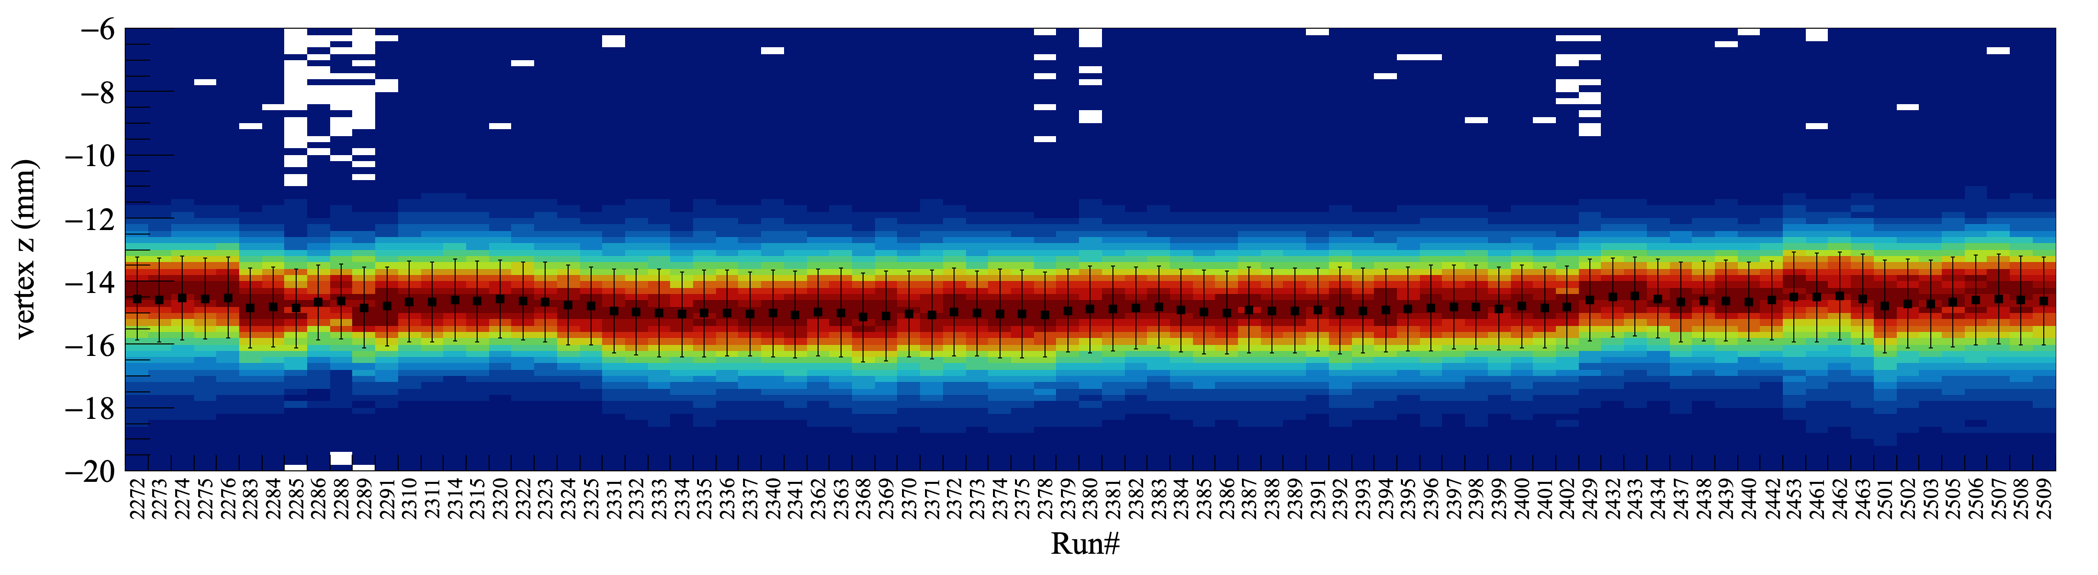
\includegraphics[width=\textwidth]{vertex-Sn108.png} 
        \caption{$\tin{108}{124}$ vertex distributon for all runs.} \label{fig:vertex108}
    \end{subfigure}
    \hfill
    \begin{subfigure}[t]{\textwidth}
        \centering
        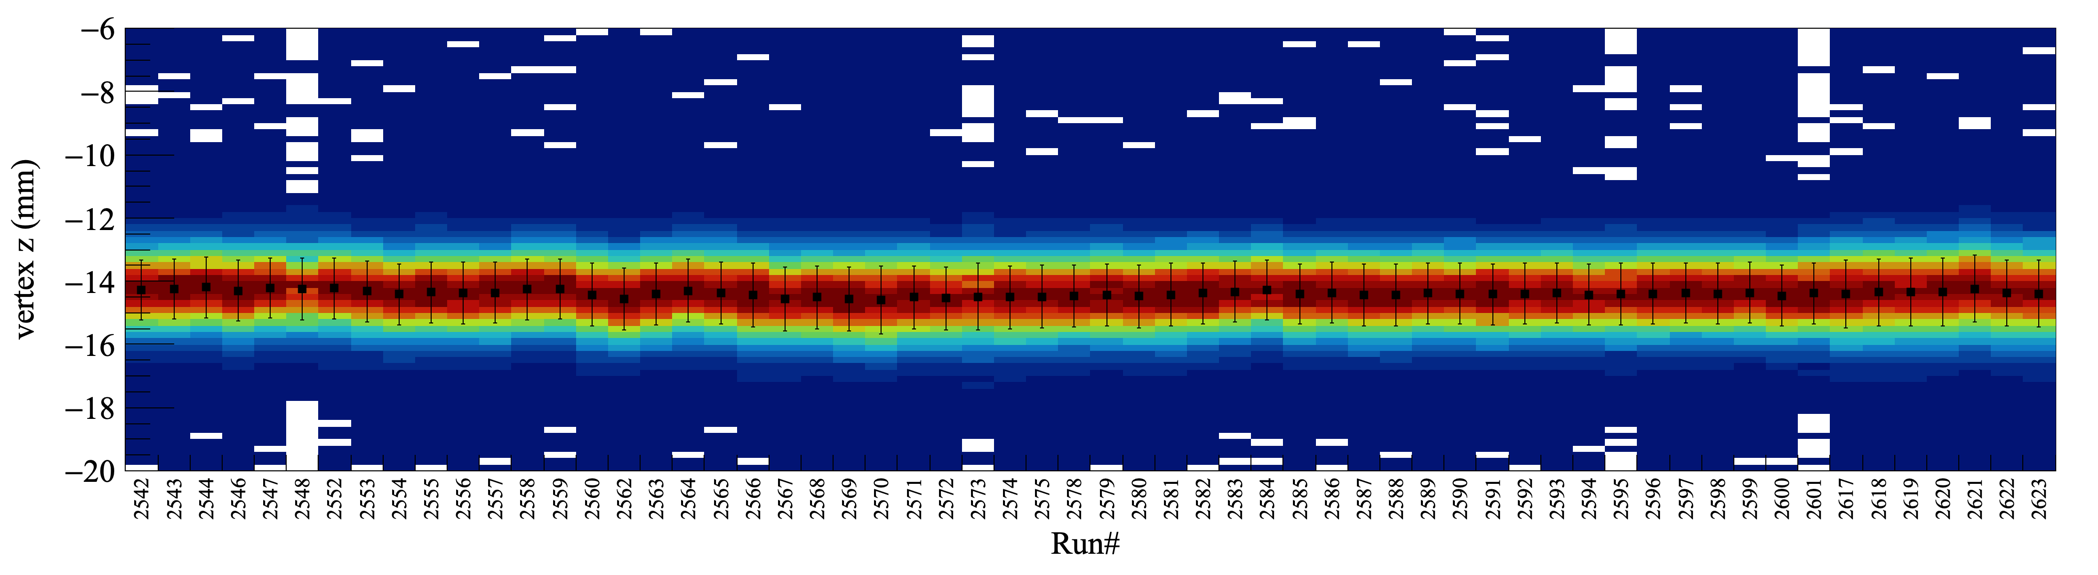
\includegraphics[width=\textwidth]{vertex-Sn112.png} 
        \caption{$\tin{112}{124}$ vertex distributon for all runs.} \label{fig:vertex112}
    \end{subfigure}
    
    \begin{subfigure}[t]{\textwidth}
        \centering
        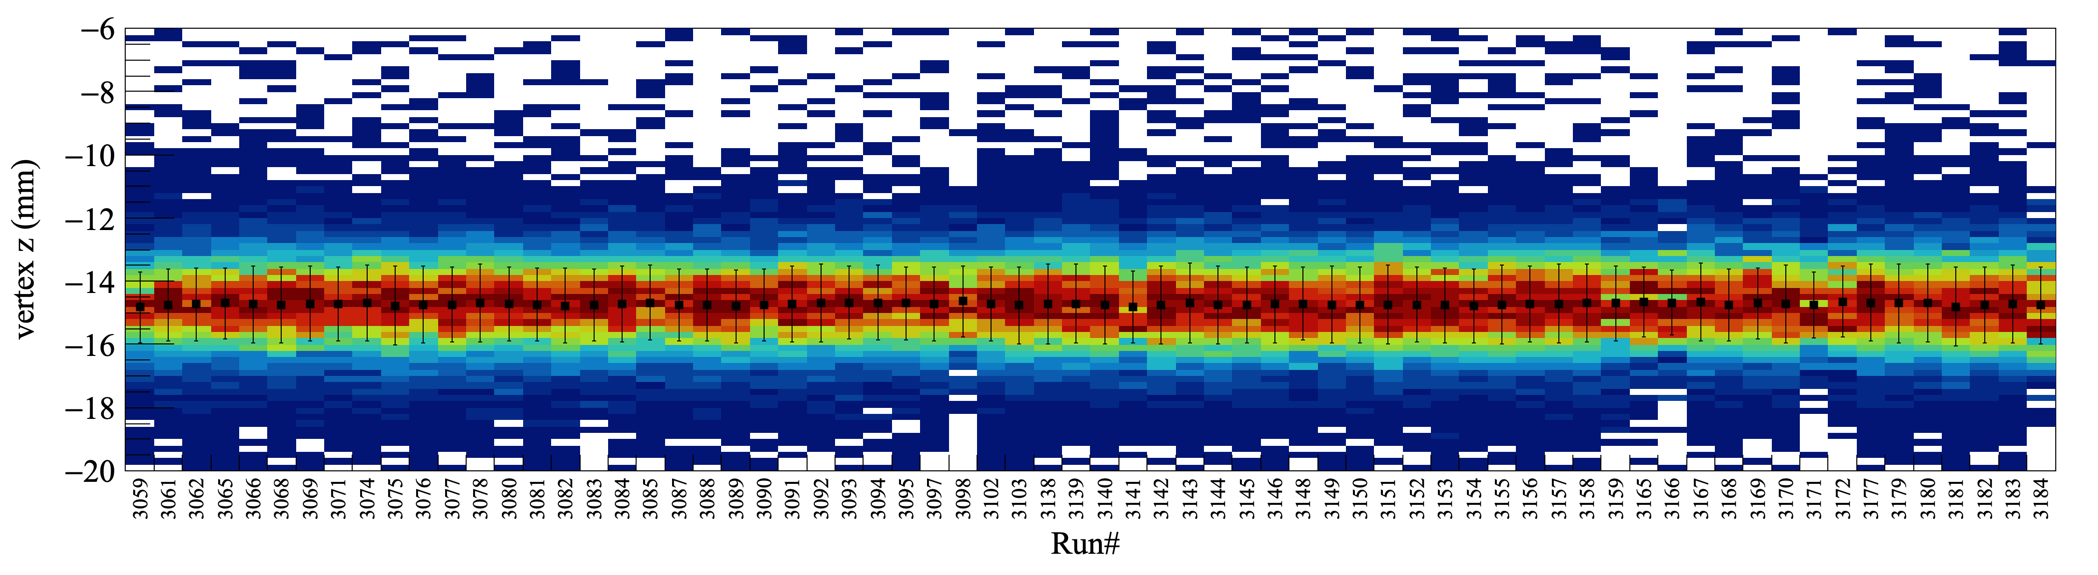
\includegraphics[width=\textwidth]{vertex-Sn124.png} 
        \caption{$\tin{124}{112}$ vertex distributon for all runs.} \label{fig:vertex124}
    \end{subfigure}
    \hfill
    \begin{subfigure}[t]{\textwidth}
        \centering
        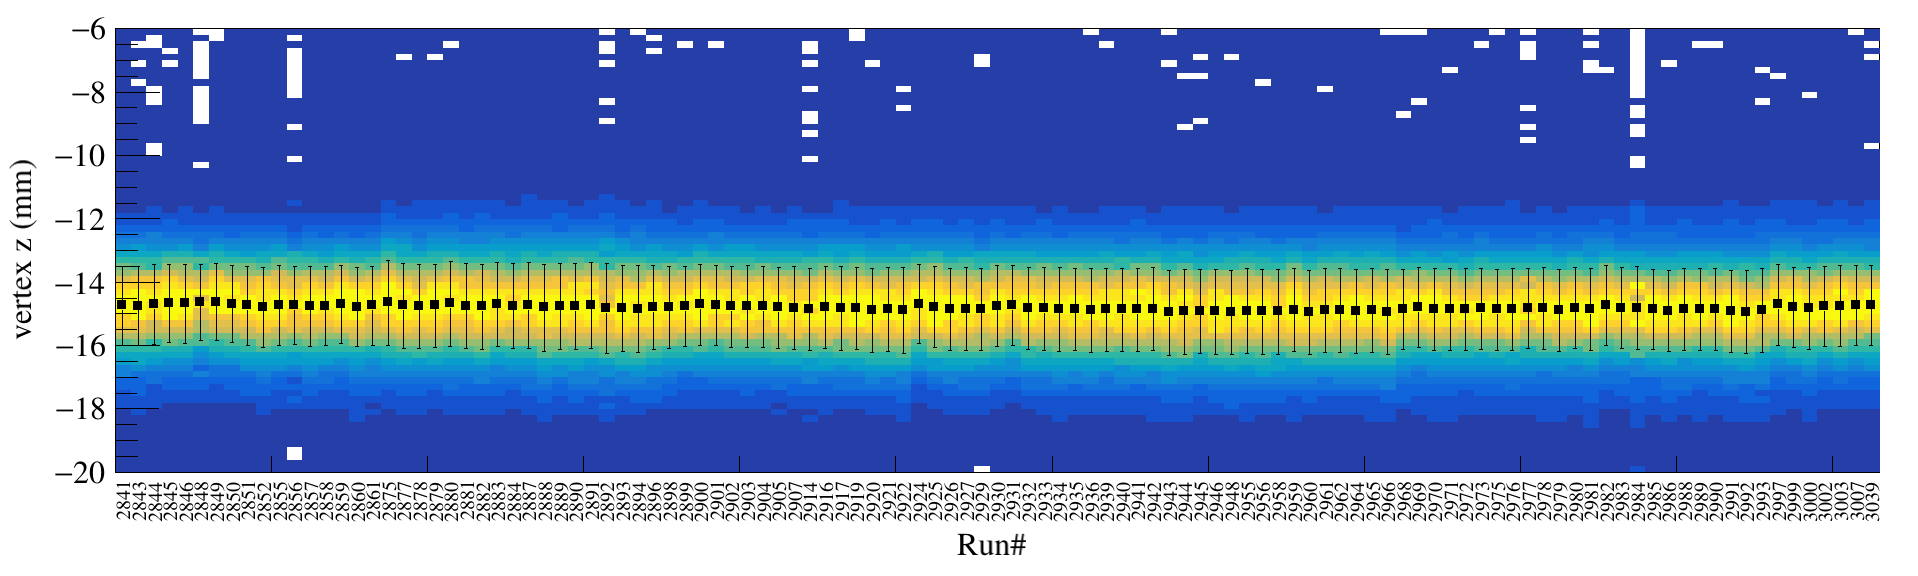
\includegraphics[width=\textwidth]{vertex-Sn132.png} 
        \caption{$\tin{132}{124}$ vertex distributon for all runs.} \label{fig:vertex132}
    \end{subfigure}
\caption{}
\label{fig:vertexdist}
\end{figure}

The vertex information of an event, described in \ref{sec:vertex}, is estimated from reconstructing the tracks of an event to one common source. The secondary beam encounters several solid and gaseous materials were a nuclear reaction can occur anywhere along the beam line. Figure~\ref{fig:overviewVertex} shows the z component of the reconstructed vertex for all events in the ${}^{132}$Sn system. Several peaks are seen in the spectrum which correspond to several dense materials in the beam line such as the entrance windows, target frame, Active Veto, with the largest peak representing the target. Also collisions happen with the detector gas inside the TPC volume which are typically called active target events. To ensure that the secondary beam is really on the target of choice we perform a vertex cut around where we believe the vertex location of the target to be.
 
 The target position was measured to be \SI{-13.2}{\milli\metre}. The z-component of all runs in each beam type are plotted around the the target region in Fig.~\ref{fig:vertexdist}. The mean position of the vertex from the reconstructed data is around \SI{-14.76}{\milli\metre} which is about \SI{1.6}{\milli\metre} off from the expected target position. The mean position for each system is listed in Table~\ref{tb:vertexresol}. Since the target thickness was less than \SI{1}{\milli\metre} for all targets. Neglecting the small distributions in the thin target, the measured width of the vertex distribution can be interpreted directly as the vertex resolution of the TPC. The extracted vertex resolutions of each system are summarized in Table~\ref{tb:vertexresol}, with an average vertex resolution of \SI{1.2}{\centi\metre}. The difference between the measured and actual target location is 10 times smaller than the intrinsic vertex resolution of the detector and is really and insignificant difference.  



\begin{table*}\centering
\ra{1.3}
\begin{tabular}{@{}rrr@{}}\toprule
\multicolumn{3}{c}{Vertex Resolution}\\
\cmidrule{1-3}
System & Mean (cm) & Sigma (cm) \\
\midrule
$\tin{132}{124}$ & -14.79  & 1.2 \\
$\tin{124}{112}$ & -14.71  & 1.1 \\
$\tin{112}{124}$ & -14.78  & 1.2 \\
$\tin{108}{112}$ & -14.75  & 1.3 \\ 
\bottomrule
\end{tabular}
\caption{Summary of measured verticies and their resolution.}
\label{tb:vertexresol}
\end{table*}


\clearpage

\section{Impact Parameter Selection}

\begin{figure}[htb]
\centering
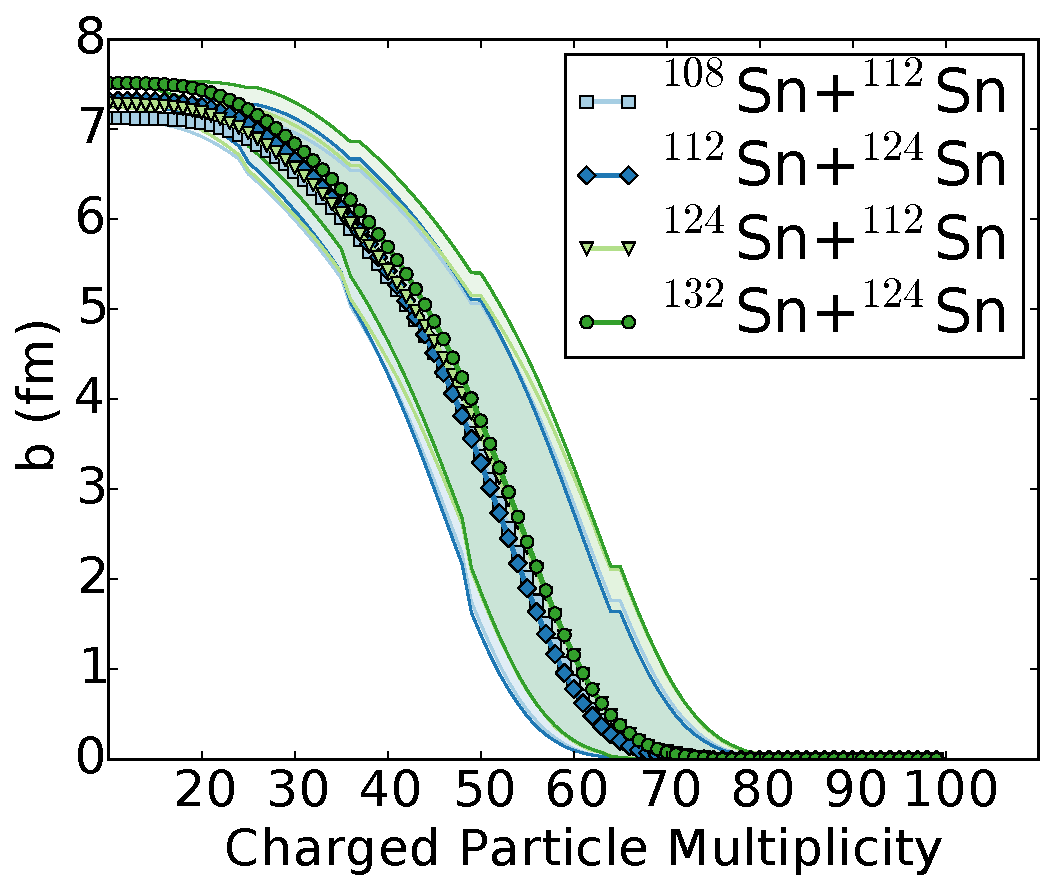
\includegraphics[scale=.5]{error_b_full.pdf}
\caption{Estimate of the impact parameter from the track multiplicity.}
\label{fig:impactPar}
\end{figure}

The impact parameter is a theoretical quantity defined as the distance, between two centers of colliding nuclei. Though there is no way to directly measure the impact parameter in an experiment, the track multiplicity can be indirectly related to the estimated impact parameter of a collision \cite{impactpar}. As discussed in Section \ref{sec:kyoto}, the Kyoto multiplicity array was used to experimentally trigger on central nuclear collision events. This is under the assumption that as the number of charged particles produced in collision is related to the overlap region of the two nuclei. This is best described by a spectator-participant model of nuclear collisions, where a large fraction of the participating nucleons in the overlap region of the two colliding nuclei fragment into individual and clusters of nucleons. In the case where the impact parameter is zero, all the nucleons in both nuclei participate, were as larger impact parameters -- more peripheral collisions -- less nucleons participate. 


%Certainly the Kyoto array introduces a bias in our measurement of the multiplicity of all the events. At low track multiplicities, the orientation of the event starts to play a major role. Theoretically the orientation of the event (the reaction plane) is random, but due to the fact that we only measure the multiplicity on the sides of the TPC, we are preferentially triggering on events with reaction planes that emit particles in these directions. Therefore events with low track multiplicity (therefore more peripheral), that emit preferentially up and down in the TPC will not be triggered on. This becomes less of an issue as even in mid-peripheral collisions were the number of particles emitted becomes much greater than the Kyoto multiplicity selection

The geometric cross section $\sigma$ can be described as, 

\begin{equation}
\sigma = \pi \cdot b^2,
\label{eq:crossSect}
\end{equation}

where $b$ is the impact parameter of the collision.  If the track multiplicity of an event $N_C$ is monotonically related to the cross section, the impact parameter can be written as a reduced impact parameter $\hat{b}$ as,
\begin{equation}
\hat{b} =  \frac{b}{b_{max}} = \int^{\infty}_{N_C} \frac{dP(N_C)}{dN_C} dN_C,
\end{equation}

where $b_{\mathrm{max}}$ represents the maximum impact parameter detected by the TPC, $b$ is the impact parameter of the vent,  and $dP(N_C/dN_C$ is the normalized multiplicity distribution \cite{reducedimpact}. The reduced impact parameter ranges from $\hat{b}=0$ for the most central collisions and to $\hat{b}=1$ for the most peripheral. A  detailed analysis was performed, determining the maximum cross section $\sigma_{max}$, for each system, in which $b_{\mathrm{max} = \sqrt{\sigma_{max}/\pi}}$. The detailed analysis is given in \cite{jon}. Figure~\ref{fig:impactPar} shows the estimated impact parameter for a given track multiplicity with the estimated error bands for each system. 

In the $\tin{132}{124}$ system the multiplicity cut was $N_C > 50$ corresponding to $\hat{b} = 0.4$ and $b = \SI{3.1}{\femto\metre}$. For the $\tin{108}{112}$ system the multiplicity cut was $N_C > 49$ corresponding to $\hat{b} = 0.4$ and $b = \SI{3.1}{\femto\metre}$. These values were averaged over the multiplicity distribution as,

\begin{equation}
 \overline{X} = \int_{N_C}^{\infty} X\frac{dP(N_C)}{dN_C} dN_C
\end{equation}

where X can be the variables $b$, $\hat{b}$. In the $\tin{132}{124}$ system the average $\overline{\hat{b}} = \num{.1(1)}$ and $\overline{b} = \SI{3}{\femto\metre}$. In the $\tin{108}{112}$ system the average $\overline{\hat{b}} = .1$ and $\overline{b} = \SI{3}{\femto\metre}$. These quantities are useful when comparing to theory. 

\section{Track Quality Cuts}
%graphic showing distance to vertex, number of clusters
%number of cluster cut
%distance to vertex
In this section we will discuss cuts which address the quality of the reconstructed track, in the following we will simply refer this as the ``track quality". Assuming tracks are mostly continuous in clusters, i.e. only randomly missing a few clusters, the number of clusters is directly related to the momentum resolution of a track. Tracks with more clusters correspond to better PID and momentum resolution. Upward-going and downward-going tracks, at larger values of $\theta_{Lab}$ are limited by the vertical space of the TPC. In these regions the track length is short and there are few clusters which are reconstructed. This leads to the low efficiency in these regions as discussed earlier in Sec.~\ref{sec:efficiency}. A cut where tracks with the number of clusters $N_{cl} > 20$ are considered quality tracks. Later in Section~\ref{sec:cutvar} the exact choice of the number 20 is discussed in more detail.

\begin{figure}[!htb]
\centering
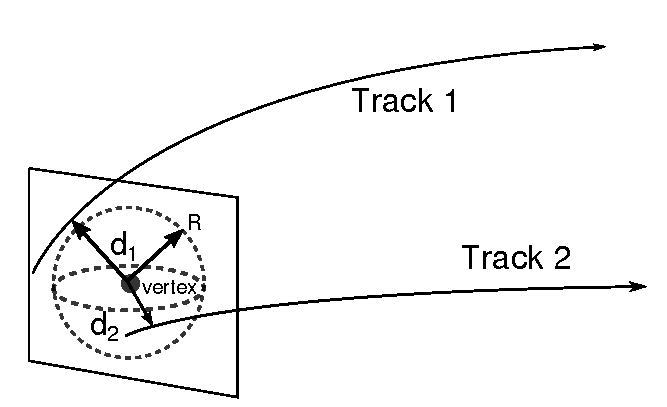
\includegraphics[scale=1.]{distancetovertex.pdf}
\label{fig:poca}
\caption{Distance to vertex for tracks.}
\end{figure}

For very long tracks, such as low momentum pions, which can make a complete circular path in the TPC, it can happen that the software incorrectly identifies the track as several separate tracks. This can happen due to discontinuities in the track due to missing hits from low energy loss, shadowing due to saturation, or possibly the software algorithm itself. Of course including all of the tracks would be counting the track several times over, and would lead to incorrect particle yields. The software will occasionally associate random disassociated clusters and construct a false track, or a so called ``ghost track". These type of tracks contribute to the background in the PID. In both of the situation of the false track or in the case of a split track the false track origin cannot be traced back to anywhere near the vertex of the event, and the distance-Of-Closest-Approach (dOCA) between the track and vertex is very large. 

To reduce the number of false tracks, a simple cut on the dOCA can be used. The vector representing the minimum distance to vertex for each track can be calculated and its corresponding magnitude. We define the distance to vertex cut as a small sphere centered around the vertex location with a some radius $R$. If the dOCA of a particular track $d_i < R$, the track is assumed to have originated from the vertex; tracks outside of the cut are thrown out of the analysis. 






\section{Angular Quality Cuts}

Since the TPC does not have spherical symmetry, there are geometric constraints and considerations that effect the efficiency of track reconstruction. Most notably upward and downward-going tracks will have the shortest track length and will correspond to low regions of efficiency as seen in \ref{sec:efficiency}. The relevant geometries which determine these regions are the corners of the field cage. Figure~\ref{fig:angleEffExplanation} shows a cartoon drawing of the front of the field cage were the angles of each corner is given. Since the window to the field cage was slightly higher, the upper angles are slightly smaller than the lower angles. These angles are actually the same as the spherical $\phi$ angle, where the left and right, most efficient regions, correspond to  $\ang{0}\substack{+24 \\ -34}$ and $\ang{180}\substack{+34 \\ -24}$.  While the exact area of zero efficiency depends on polar angle $\theta_{Lab}$, a clear cut off around these angles can be seen in Fig.~\ref{fig:angleEffExplanation} in the angular distribution of the measured tracks, where the experimental data was fitted with a Fermi distribution to find the inflection point of where the efficiency drops off significantly. The angular cuts applied to the data is listed by particle type in Table~\ref{tb:anglecuts}. The values are very similar to the simple calculation that was outlined above. 


\begin{figure}[!htb]
\centering
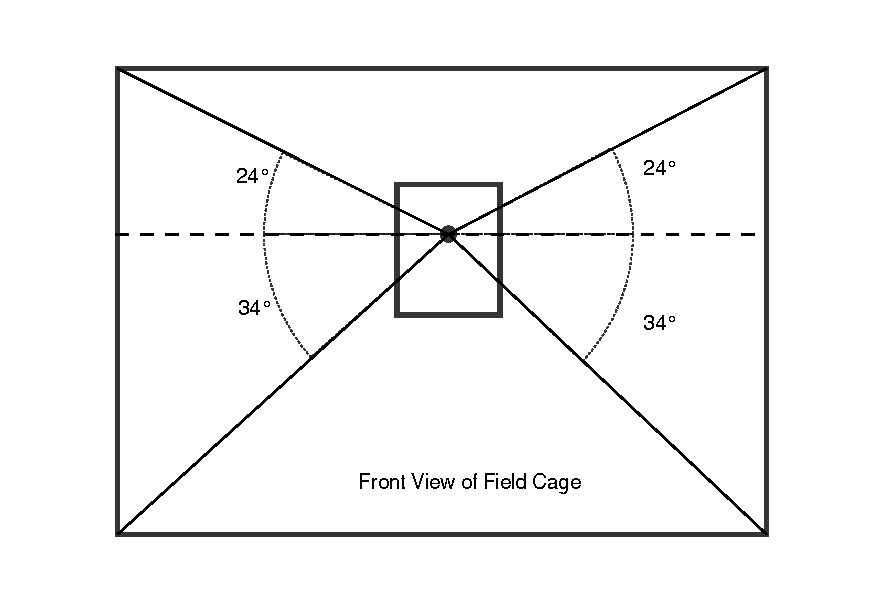
\includegraphics[scale=.75]{tpcAngle.pdf}
\caption{Rough Geometry of the TPC field cage.}
\label{fig:angleEffExplanation}
\end{figure}


\begin{figure}[!htb]
     \centering
     \begin{subfigure}[b]{0.49\textwidth}
         \centering
         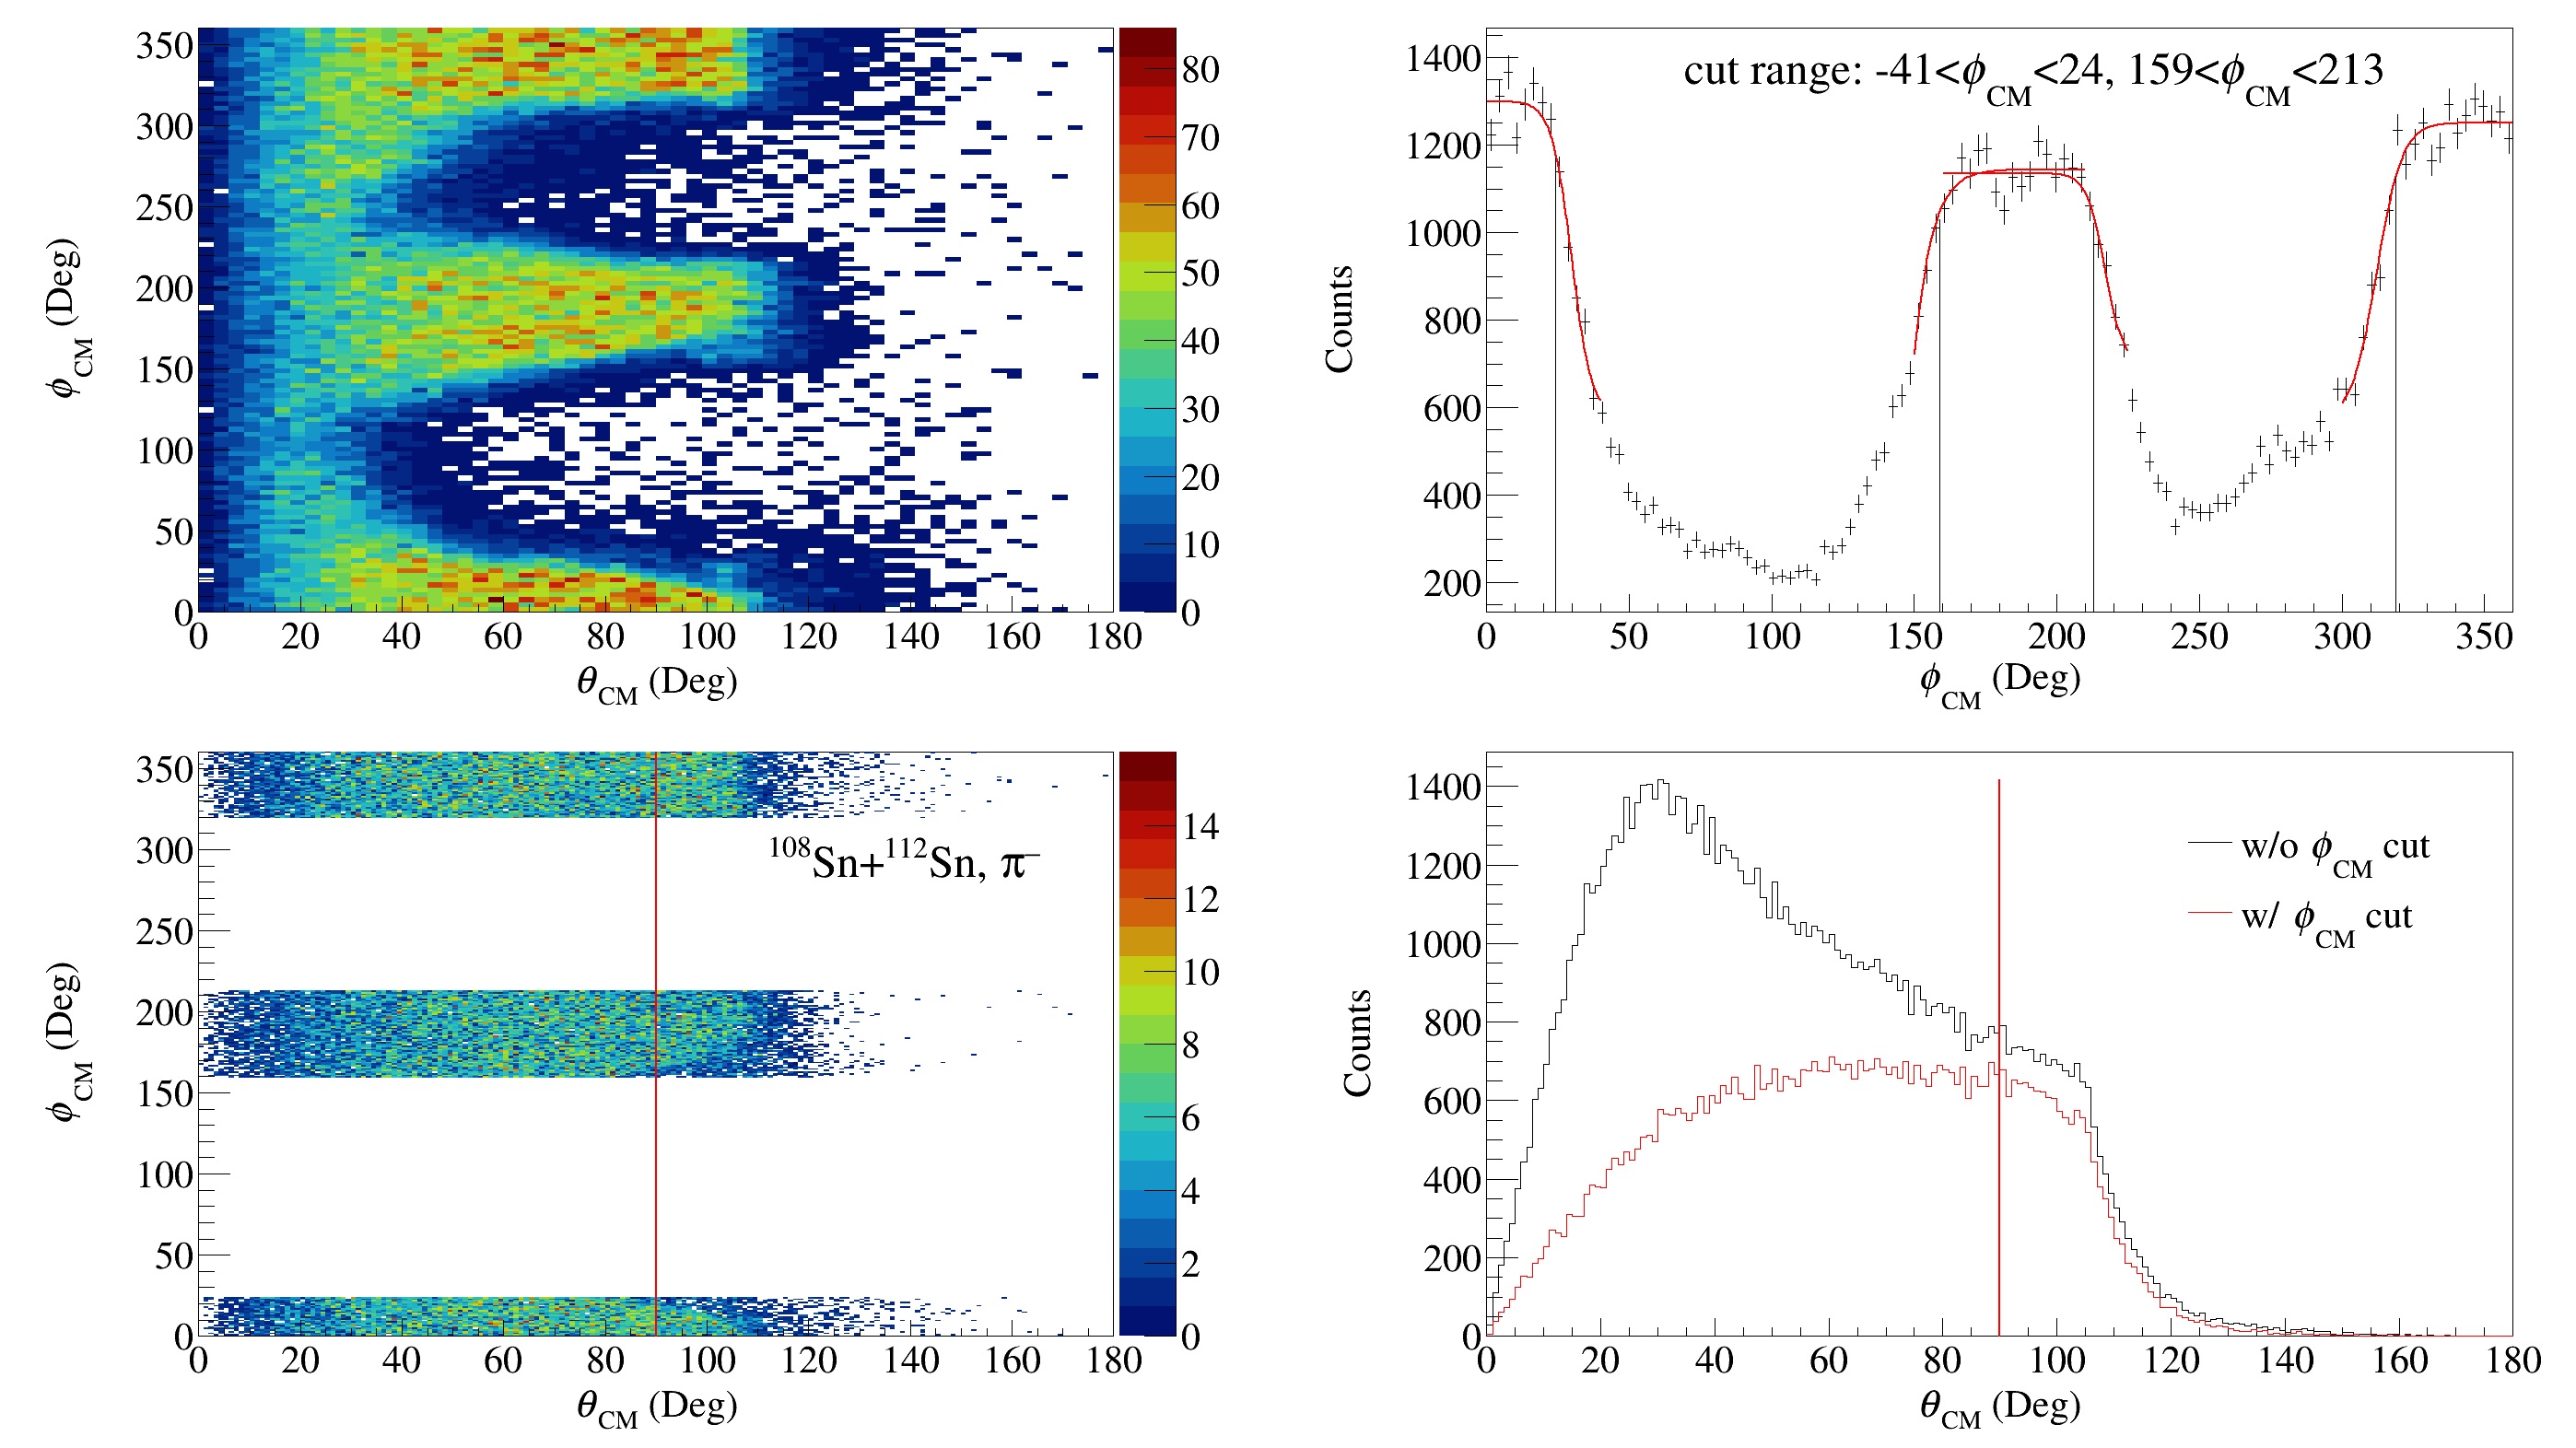
\includegraphics[width=\textwidth]{angularCut-pim-Sn108.png}
         \caption{$y=x$}
         \label{fig:pim108angle}
     \end{subfigure}
     \hfill
     \begin{subfigure}[b]{0.49\textwidth}
         \centering
         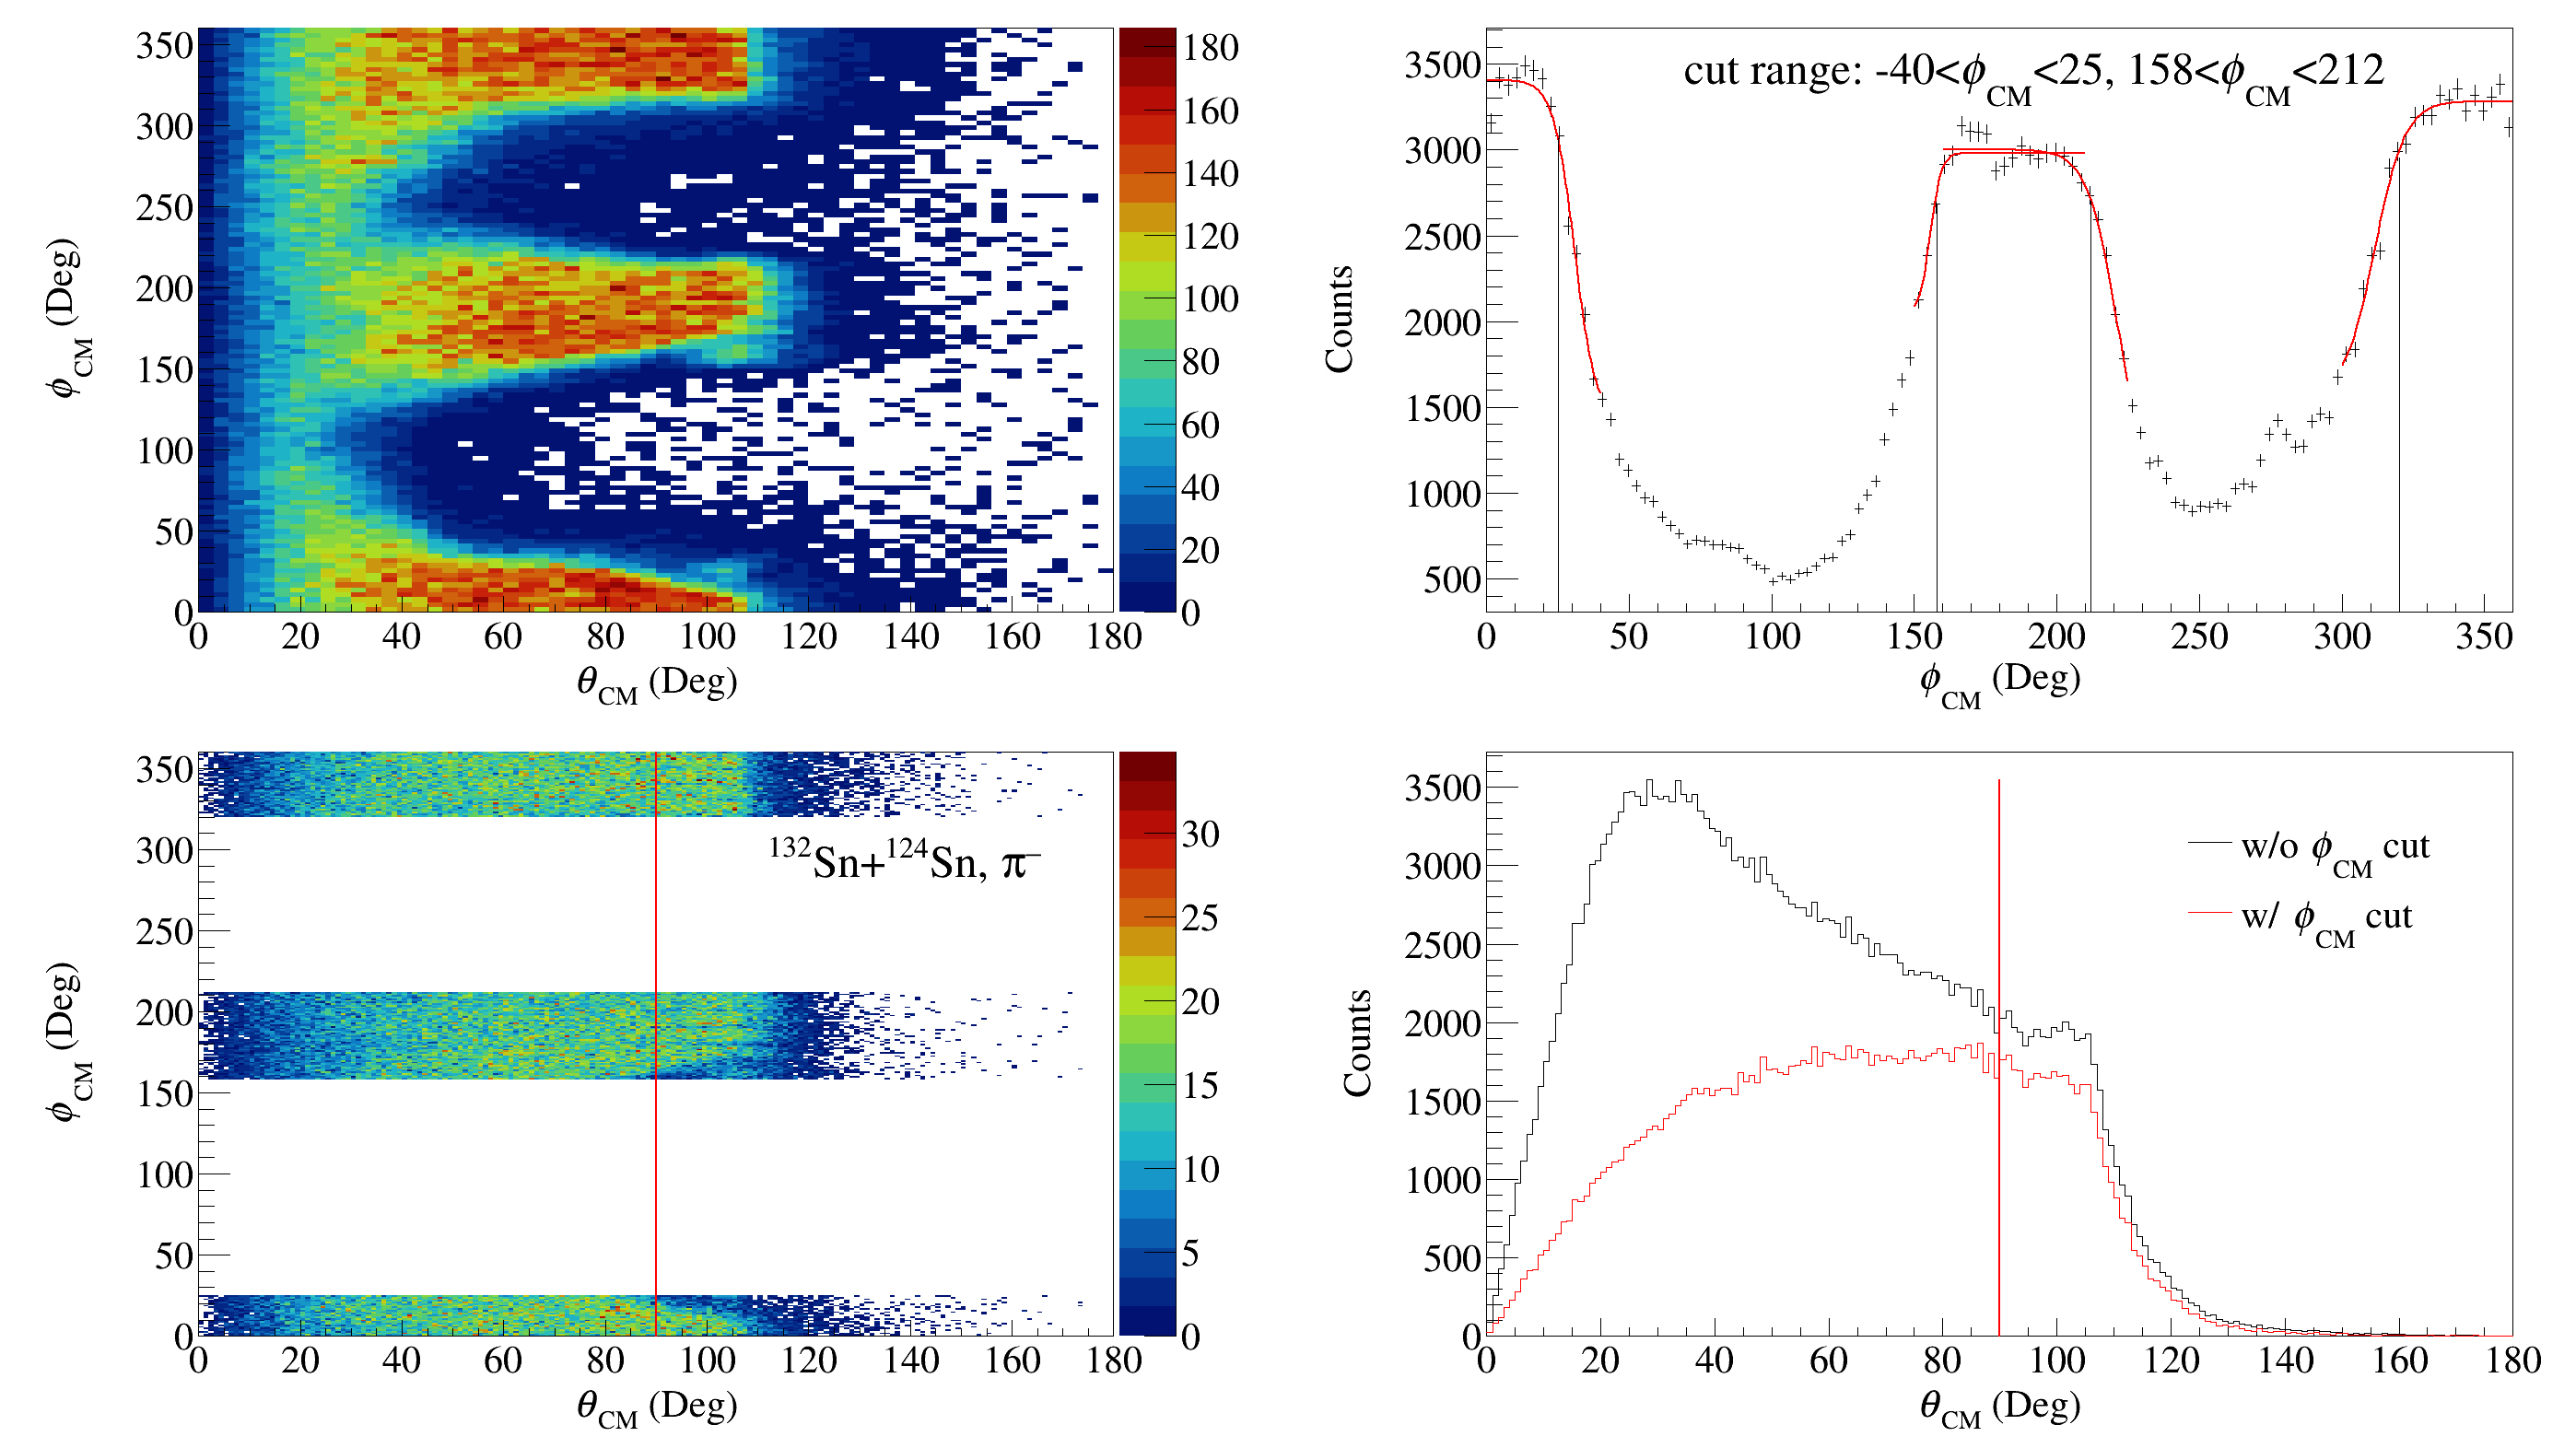
\includegraphics[width=\textwidth]{angularCut-pim-Sn132.png}
         \caption{$\tin{132}{124}$ $\pi^-$ angular spectra.}
         \label{fig:pim132angle}
     \end{subfigure}
        \caption{Three simple graphs}
        \label{fig:pim}
\end{figure}


\begin{figure}[!htb]
     \centering
     \begin{subfigure}[b]{0.49\textwidth}
         \centering
         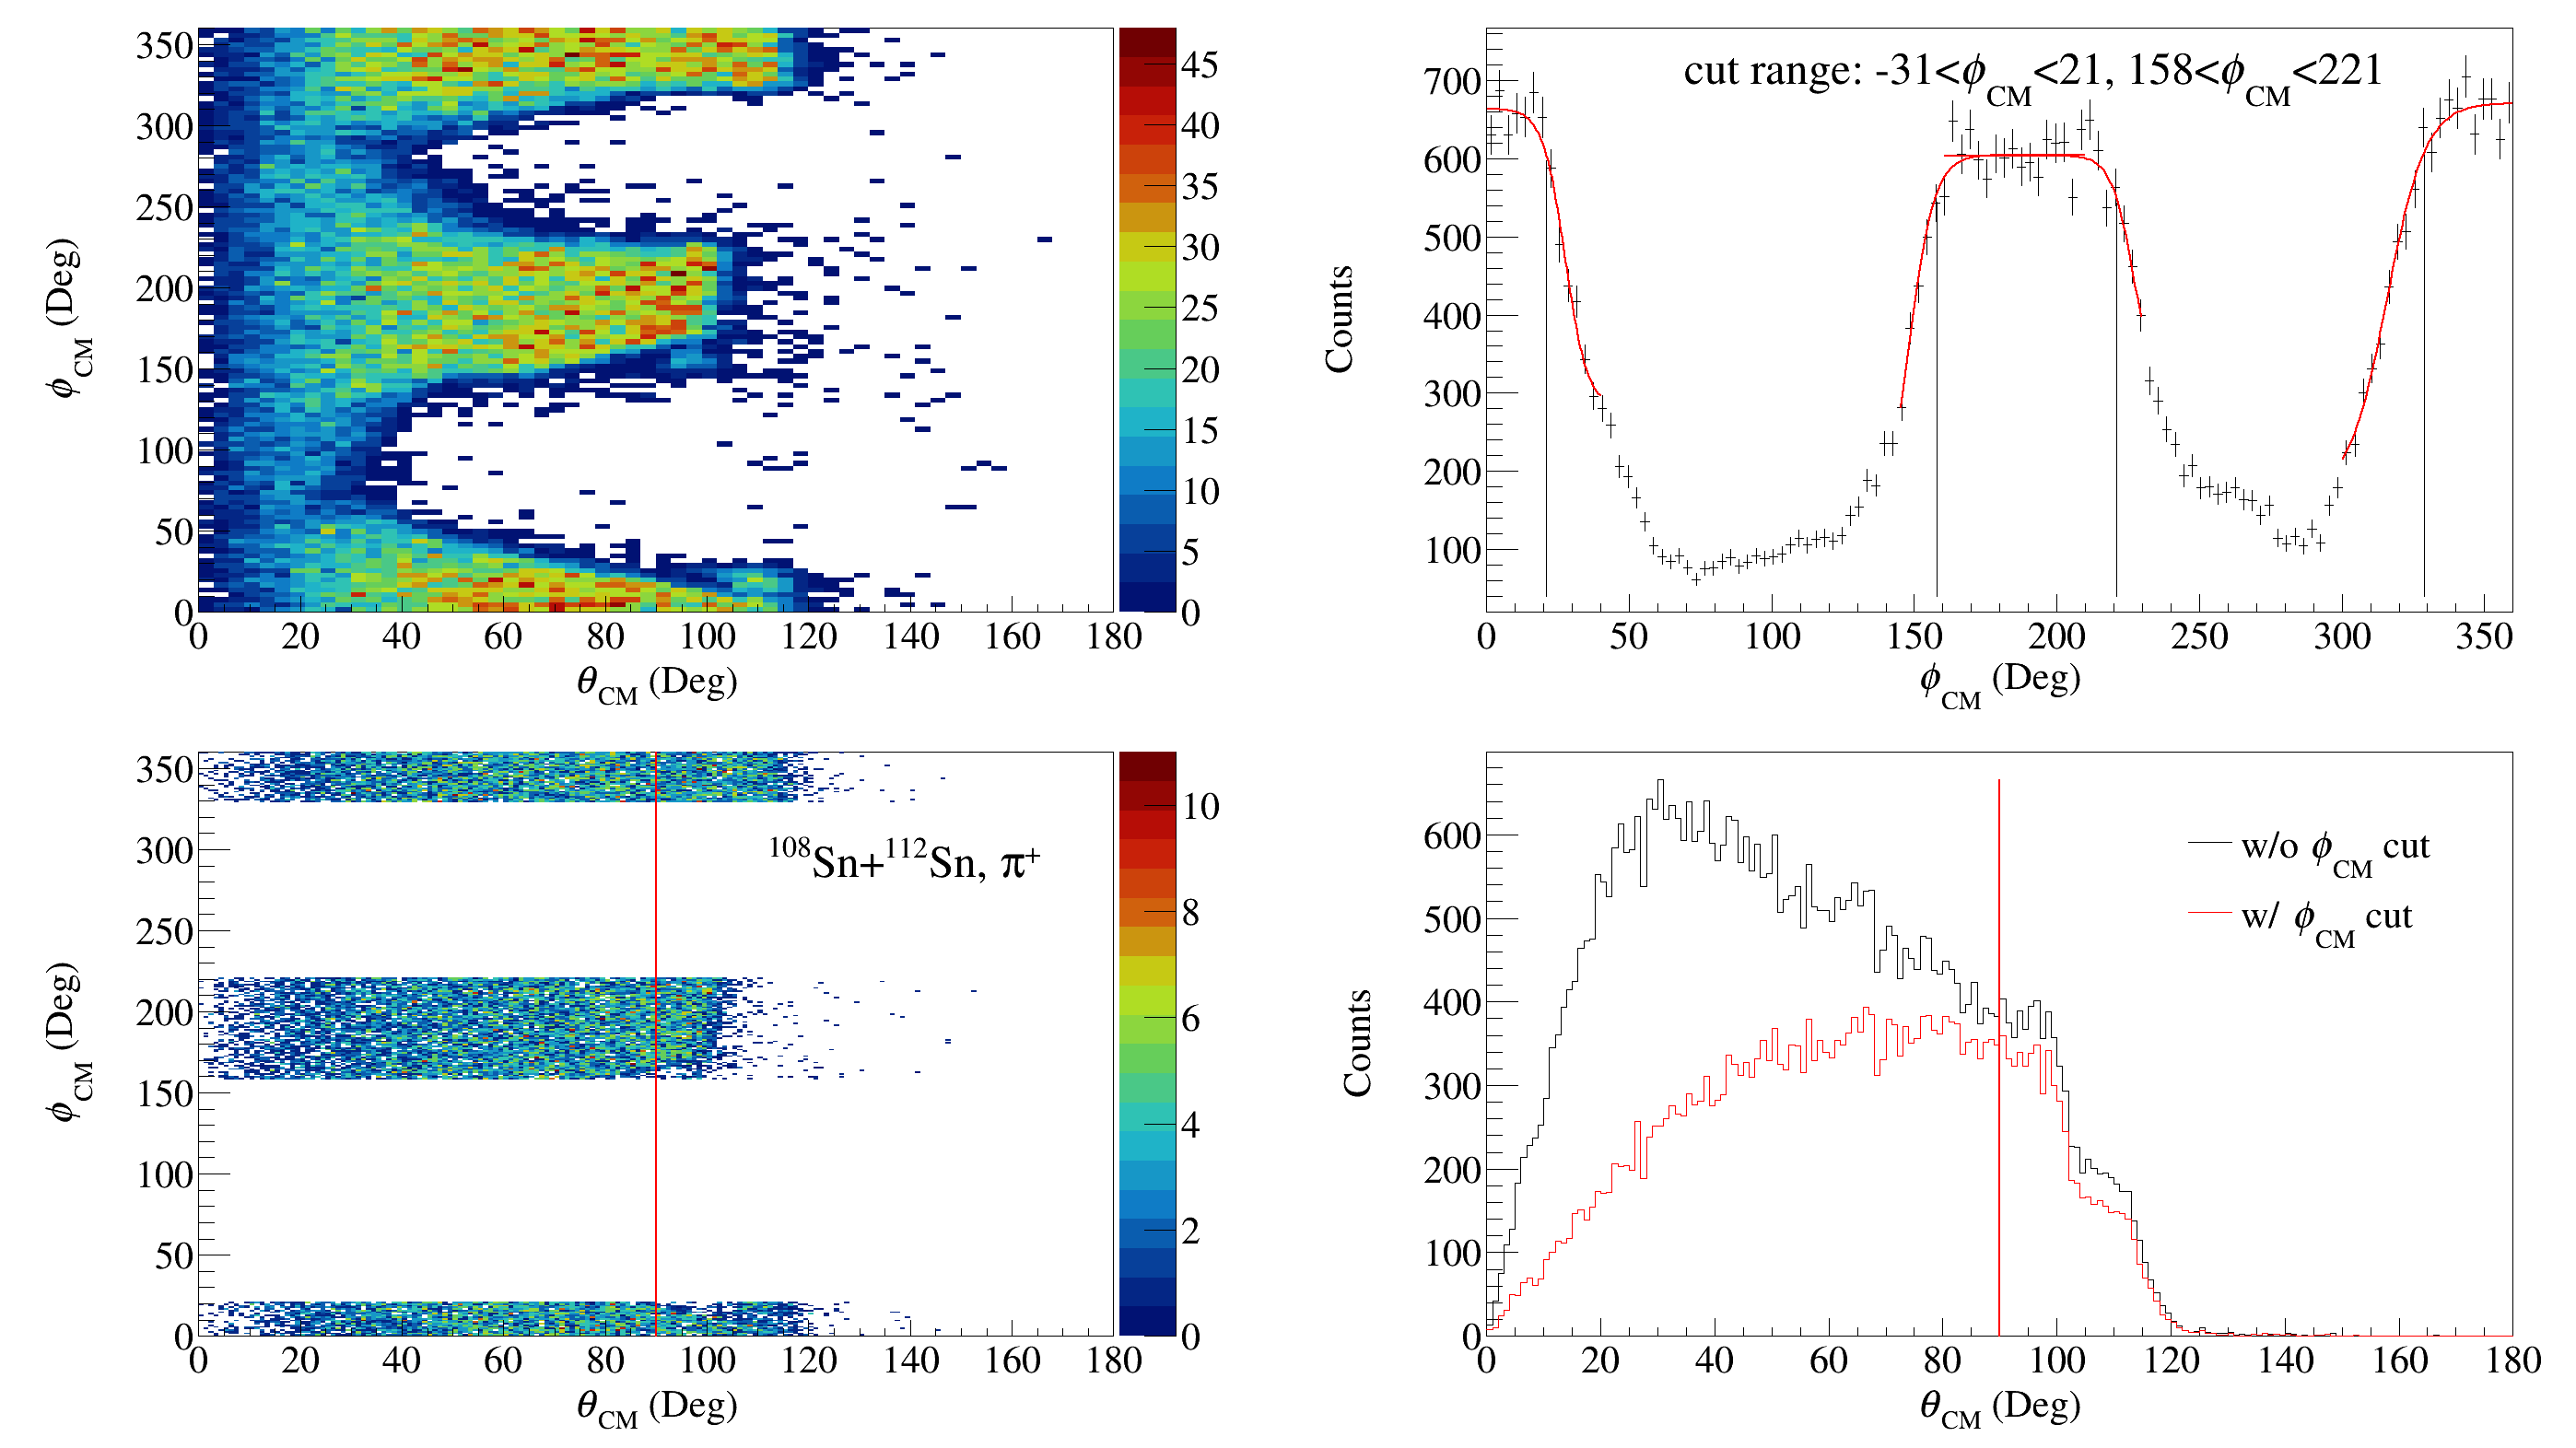
\includegraphics[width=\textwidth]{angularCut-pip-Sn108.png}
         \caption{$\tin{108}{112}$ $\pi^-$ angular spectra.}
         \label{fig:pip108angle}
     \end{subfigure}
     \hfill
     \begin{subfigure}[b]{0.49\textwidth}
         \centering
         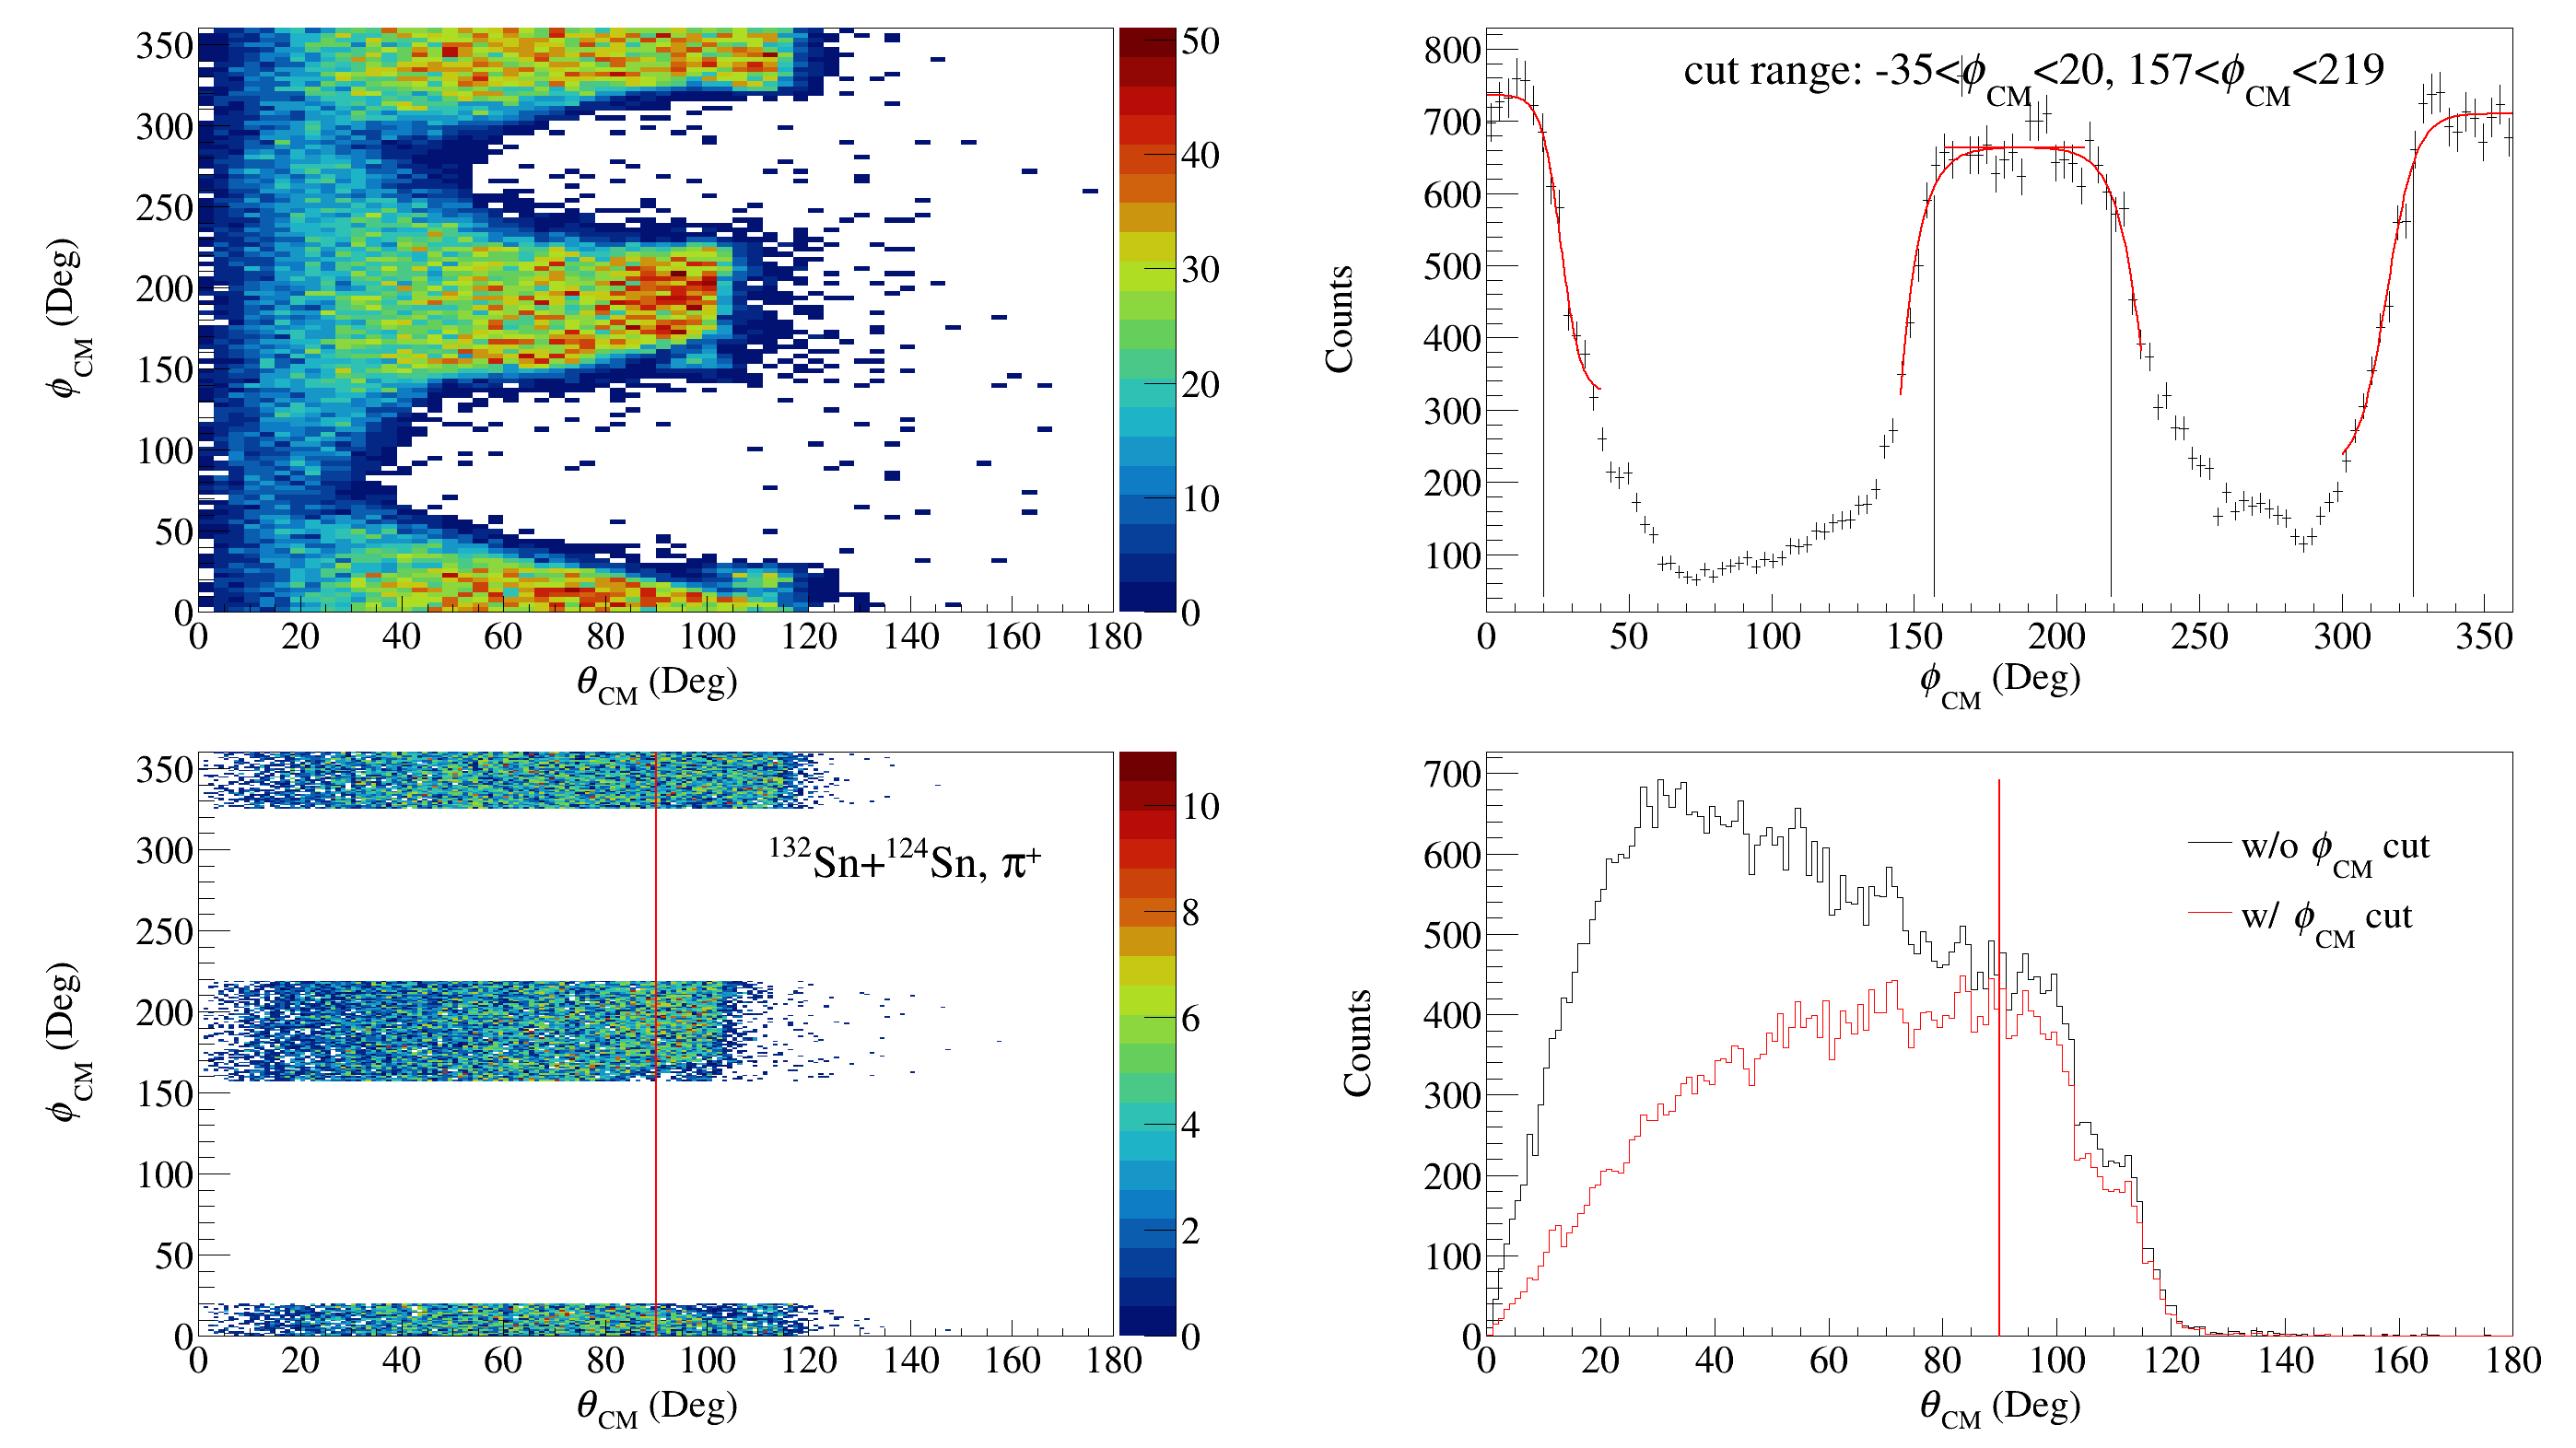
\includegraphics[width=\textwidth]{angularCut-pip-Sn132.png}
         \caption{$\tin{132}{124}$ $\pi^-$ angular spectra.}
         \label{fig:pip132angle}
     \end{subfigure}
        \caption{Three simple graphs}
        \label{fig:pip}
\end{figure}



 \begin{table*}[!htb]
 \centering
\ra{1.3}
\begin{tabular}{@{}ccc@{}}\toprule 
Particle Type & $\theta_{CM}$ cut & $\phi$ cut  \\ [0.5ex] 
 \midrule
$\pi^+$  & $\theta_{CM}$ < \ang{90}   &  \ang{-35} < $\phi$ < \ang{20} $\cap$ \ang{157} < $\phi$ < \ang{219}  \\
$\pi^-$  & $\theta_{CM}$ < \ang{90}   &  \ang{-40} < $\phi$ < \ang{25} $\cap$ \ang{158} < $\phi$ < \ang{212}   \\
 \bottomrule
\end{tabular}
\caption{Angular cuts for each system and particle type}
\label{tb:anglecuts}
\end{table*}



These regions can also be seen in the earlier discussion in the MC embedded efficiency in Fig.~\ref{fig:pim_eff_ex}.  We could of course include a larger region where the efficiency is small but not zero but it is good practice not to efficiency correct already small numbers with small efficiency values. The solid angle covered by the cut is written as,

\begin{equation}
\Delta\Omega = \Delta\phi(\cos(\theta_1) - \cos(\theta_2)),
\end{equation}

where $\Delta\phi = (\phi_2 - \phi_1)$  and $\theta_{1,2}$ are the $\theta$ angle cuts, in units of \si{\radian}. The solid angle covered by the $\pi^-$ cuts is \SI{2.077}{\steradian} and for $\pi^+$ cuts \SI{2.042}{\steradian}. Assuming the pion emission is isotropic, we multiply each observed pion by a correction factor, $C_a$, to correct for the full 4$\pi$ angular coverage, 

\begin{equation}
C_a = \frac{4\pi}{\Delta\Omega},
\end{equation}

for $\pi^+$ that is \num{6.15} and $\pi^-$ \num{6.05}. We assume the pion emission is isotropic for a couple of reasons. The symmetry of very central collisions is invariant with respects to any rotations. Also the mass of the pion is smaller than the nucleons mass and therefore collective motion leading to anisotropies would be small for the pion, i.e. most of the motion would be thermal. We also measured two systems $\tin{112}{124}$ and its inverse $\tin{124}{112}$. The forward emission in the $\tin{124}{112}$ system is really the same as the backward emission of the $\tin{112}{124}$ system and vice versa. It was shown for pions emitted in central collisions the forward and backward emission was the same \cite{jon}, proving that at least for central collisions pions are emitted isotropically to a good approximation. 


